%%This is a very basic article template.
%%There is just one section and two subsections.
\RequirePackage[ngerman=ngerman-x-latest]{hyphsubst}
%\documentclass[11pt,a4paper]{scrbook}
\documentclass[11pt,a4paper]{scrartcl}
%\documentclass[11pt,a4paper]{article}
\usepackage[utf8]{inputenc}
\usepackage[T1]{fontenc}
%\renewcommand{\familydefault}{\sfdefault}
\usepackage[a4paper]{geometry}
%\geometry{verbose,tmargin=2.5cm,lmargin=2.5cm,rmargin=1.5cm,bmargin=3cm}
\usepackage[ngerman,english]{babel}
%\usepackage{ngerman}
\usepackage{amsmath}
\usepackage{mhchem}
\usepackage{textcomp}
\usepackage{amsfonts}
\usepackage{amssymb}
\usepackage{setspace}
\usepackage[pdftex]{graphicx}
\usepackage{epstopdf}
\usepackage[final]{pdfpages}
\usepackage{booktabs}
\usepackage{multirow}
%\usepackage{chngcntr}
%\usepackage{hyperref}0
\usepackage{placeins}

\setlength{\parindent}{0pt}
\setlength{\headheight}{14pt}
\usepackage{fancyhdr}
\pagestyle{fancy}
\begin{document}

\begin{titlepage}
\begin{center}

\includegraphics[scale=0.8]{images/HSR.pdf}
\linebreak 
\includegraphics[scale=0.3]{images/IET.pdf}
\end{center}

\vspace{2.5cm}
%\vspace{0.5cm}
\begin{center}
\textbf{Latentwärmespeicher und chemische Speicher
in Gebäudeenergieversorgungssystemen}
\linebreak
%\textbf{evtl. Vertraulich}
\end{center}
\vspace{1.8cm}
%\vspace{0.5cm}
\begin{center}
Seminararbeit
\end{center}
\vspace{1cm}
\begin{center}
\textbf{von \linebreak Dominik Strebel \linebreak Simon Boller \linebreak
Leandro Nikolic} \linebreak
\linebreak 
Abgabedatum: 23.05.2014
\linebreak
\end{center}
\vspace{3cm}
\noindent Betreuung:

\noindent Prof. Carsten Wemhöner

\noindent HSR Rapperswil

\noindent Institut für Energietechnik

\end{titlepage}
%\thispagestyle{empty}
%\cleardoublepage
\renewcommand{\footrulewidth}{0pt}
\renewcommand{\headrulewidth}{0pt}
\lhead{}
\chead{}
\rhead{}
\cfoot{} 
\selectlanguage{ngerman}


 \vspace*{12.5cm}
\begin{minipage}{80mm}
	Keywords: Wärmespeicher, Latentwärmespeicher, chemische Speicher
 \\
	\\
	Zitiervorschlag: 
	Ich beschäftige mich nicht mit dem, was getan worden ist. Mich interessiert, was getan werden muss. Marie Curie
	\vspace{1cm}


  \rule{80mm}{2pt}
  Impressum: \\
  Hochschule für Technik Rapperswil \\
  IET, Institut für Energietechnik \\ 
  Oberseestrasse 10 \\
  8640 Rapperswil\\
  \rule{80mm}{2pt}
\end{minipage}
\newpage


\tableofcontents
\newpage
\renewcommand{\headrulewidth}{0.4pt}
\renewcommand{\footrulewidth}{0.4pt}
\lhead{}
\chead{Seminararbeit}
\rhead{}
\cfoot{}
\setcounter{page}{1}
\cfoot{\thepage}
\section{Einleitung}
\newpage
\section{Allgemeiner Vergleich von chemischen, latenten und sensiblen
Wärmespeichern}
Wärmespeicher lassen sich generell in zwei verschiedene Hauptgruppen einteilen.
Einerseites existieren chemische Energiespeicher, andererseits
direkt-thermische, in denen die Energie ohne Umwandlung als thermische Energie
verfügbar ist. Eine Gliederung der verschiedenen Technologien befindet sich in
der Abbildung
\ref{fig:Wärmespeicher}

\begin{figure}[h]
\begin{center}
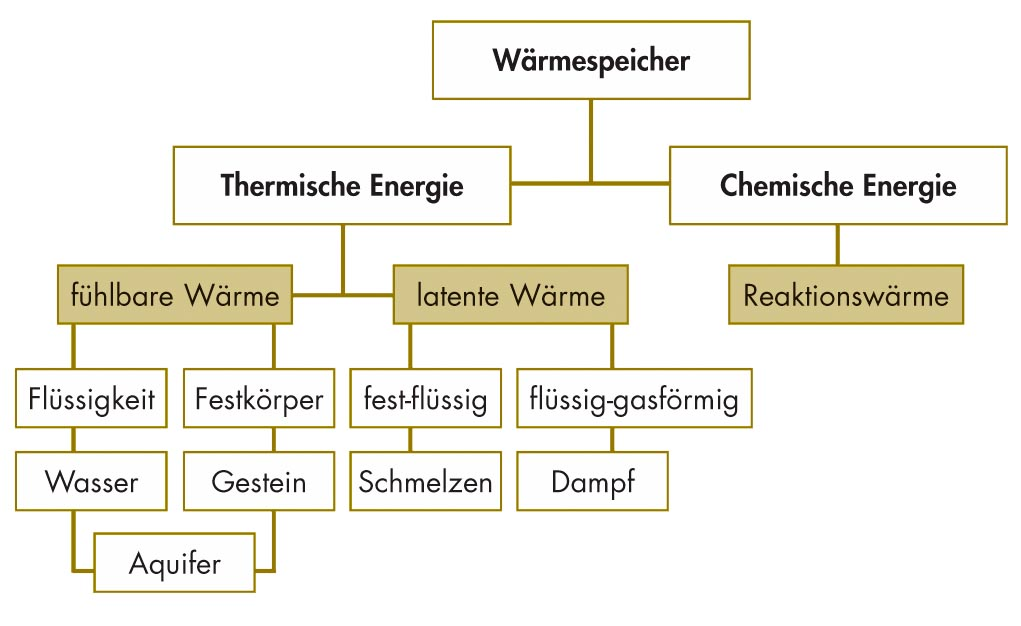
\includegraphics[scale=0.3]{images/speicher.jpg}
\caption{Übersicht über die verschiedenen Wärmespeichertechnolgien \cite{BINE1}}
\label{fig:Wärmespeicher}
\end{center}
\end{figure}


Diese verschiedenen Arten von Wärmespeichern haben natürlich auch ganz eigene Eigenschaften bezüglich Energiedichte und Einsatztemperaturen. Die Abbildung \ref{fig:temperaturenergiedichte} zeigt den Überblick. Die Abkürzungen TCM steht für Thermo Chemical Material und die PCM für Phase Change Material. Der Vergleich zeigt, dass von den fühlbaren Wärmespeicherung über die latente zur Thermochemischen Wärmespeicherung grosse unterscheide bestehen.

\begin{figure}[h]
\begin{center}
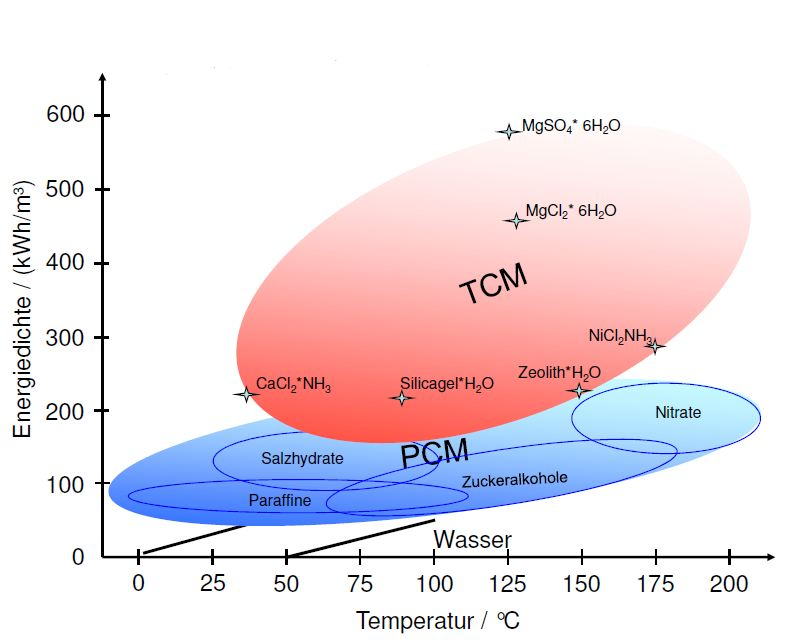
\includegraphics[scale=0.5]{images/temperaturenergiedichte.jpg}
\caption{Überblick der verschiedenen Thermischen Energiespeichern \cite{zaebayern}}
\label{fig:temperaturenergiedichte}
\end{center}
\end{figure}

\subsection{Chemische Speicher}
Chemische Speicher werden über eine chemsiche Reaktion be- und entladen. Per
Definition eines Speichers sind diese Reaktionen reversibel. Die nutzbare
Wärmeenergie entspricht der freigesetzten Reaktionsenthalpie $\Delta
H_{\mathrm{R}}$. Die Nutztemperatur des Speichers bestimmt die in Frage
kommenden chemischen Reaktionen und schränkt die zu verwenden Stoffe erheblich
ein.

Chemische Speicher werden heute im allgemeinen mit sorptiven Prozessen gebaut.
Dies ist einerseits die Adsorption, eine Anlagerung eines Gases oder einer
Flüssigkeit an einen Feststoff und andererseits die Absorption, das Lösen von
Gasen in einer Flüssigkeit. In untenstehender Gleichung ist das Grundlegende
Prinzip der Adsorption erklärt.
\begin{align}
\text{Sorbens}+nH_2O\leftrightharpoons \text{Sorbens}+nH_2O+\Delta H_{ads}
\end{align}
Nutzbar ist die freiwerdende Reaktionsenthalpie $\Delta H_{ads}$ wenn die
Reaktion nach links erfolgt. Die Beladung erfolgt nach umgekehrten Prinzip.  
\cite{Wesselak}

\subsection{Latente Speicher}
Latentwärmespeicher nutzen den Phasenübergang eines Stoffs zur Speicherung von
Wärme. Wie bei den chemischen Speichern beschränken sich die Einsatzgebiete auf
die Phasenübergangseigenschaften des Mediums. Beispielsweise erfolgt der
Phasenübergang von Wasser bei 273.15K. Die freiwerdende bzw. benötigte Energie
für einen fest-flüssig Phasenübergang bei Wasser beträgt 333.5 kJ/kg.
Aufgrund der grossen Dichteänderund der meisten flüssig-gasförmig
Phasenübergänge werden diese selten zu Speicherzwecken genutzt, obwohl die
Kondensations/Verdampfungswärme der Stoffe meistens grösser ist. Die Materialien
werden mit PCM für \flqq Phase Changing Materials\frqq{} abgekürzt.

Die speicherbare Energie ergibt sich nach

\begin{align}
\Delta E = mh_{pc}
\end{align}
Produkt von Masse und Schmelz/Kristallisationsenthalpie. Die verwendeten
Materialien lassen sich zweidimensional anhand der
Schmelz/Kristallationsenthalpie und der Schmelztemperatur kategorisieren. 

Nachteilig bei Latentwärmespeichern ist besonders, dass bei reinen Feststoffen
naturgemäss kein konvektiver Wärmetransport stattfinden kann. Dem versucht man
im heutigen Forschungskontext mit sogennaten Slurries zu begegnen. Im weiteren
Verlauf dieser Arbeit werden wir darauf noch eingehen. \cite{Wesselak}

\subsection{Sensible Wärmespeicher}

Sensible Wärmespeicher funtkionieren klassisch über eine Temperaturdifferenz
$\Delta T$. Sensibel bedeutet in diesem Kontext \flqq fühlbar\frqq{}. Die
Be- und Entladung funktioniert also über einen \flqq fühlbare\frqq{}
Temperaturdifferenz die über konvektive und konduktive Prozesse zum Austausch
führt. Als Speichermedium eignen sich aufgrund von Dichteeigenschaft und
gewünschter Konvektion verschiedene Flüssigkeiten. Die spezifische
Wärmekapazität $c$ und die Speichermasse $m$ bestimmen die Kapazität des
Speichers, der Massenstrom $\dot{m}$ und Temperaturdifferenz $\Delta T$ die
Leistung des Speichers. Aufgrund der auch an den Speicherwänden anliegenden
Temperaturdifferenz $\Delta T$ ist eine Dämmung zwingend notwendig. 

Technisch gesehen unterscheidet man zwischen Kurz- und Langzeitspeichern.
Typischer Kurzzeitspeicheranwendungen im Gebäudetechnikbereich sind
Warmwasserboiler. Die Verweildauer des Wassers beträgt hier Stunden bis maximal
Tasge. Langzeitspeicher werden zur saisonalen Wärmespeicherung genutzt. Dies
findet beim System Jenni Einsatz. Die Speicher sind so dimensioniert, dass die
SPeicherkapazität nur ein- bis wenige Male im Jahr genutzt wird. Dafür sind aber
grosse Speichermassen, bis zu 100'000l Wasser nötig.

Die gespeicherte Energiemenge lässt sich nach
\begin{align}
\Delta E = mc\Delta T = \rho Vc \Delta T
\end{align}
definieren. Wasser besitzt mit 4.19 kJ/kg/K eine hohe spezifische
Wärmekapazität und wird deshalb als kostengünstiges, effizientes und
umweltfreundliches Medium omnipräsent eingesetzt.
In Abbildung \ref{fig:Langzeitspeicher} sind die verfügbaren
Langzeitsenisbelwärmespicher abgebildet.

\begin{figure}[h]
\begin{center}
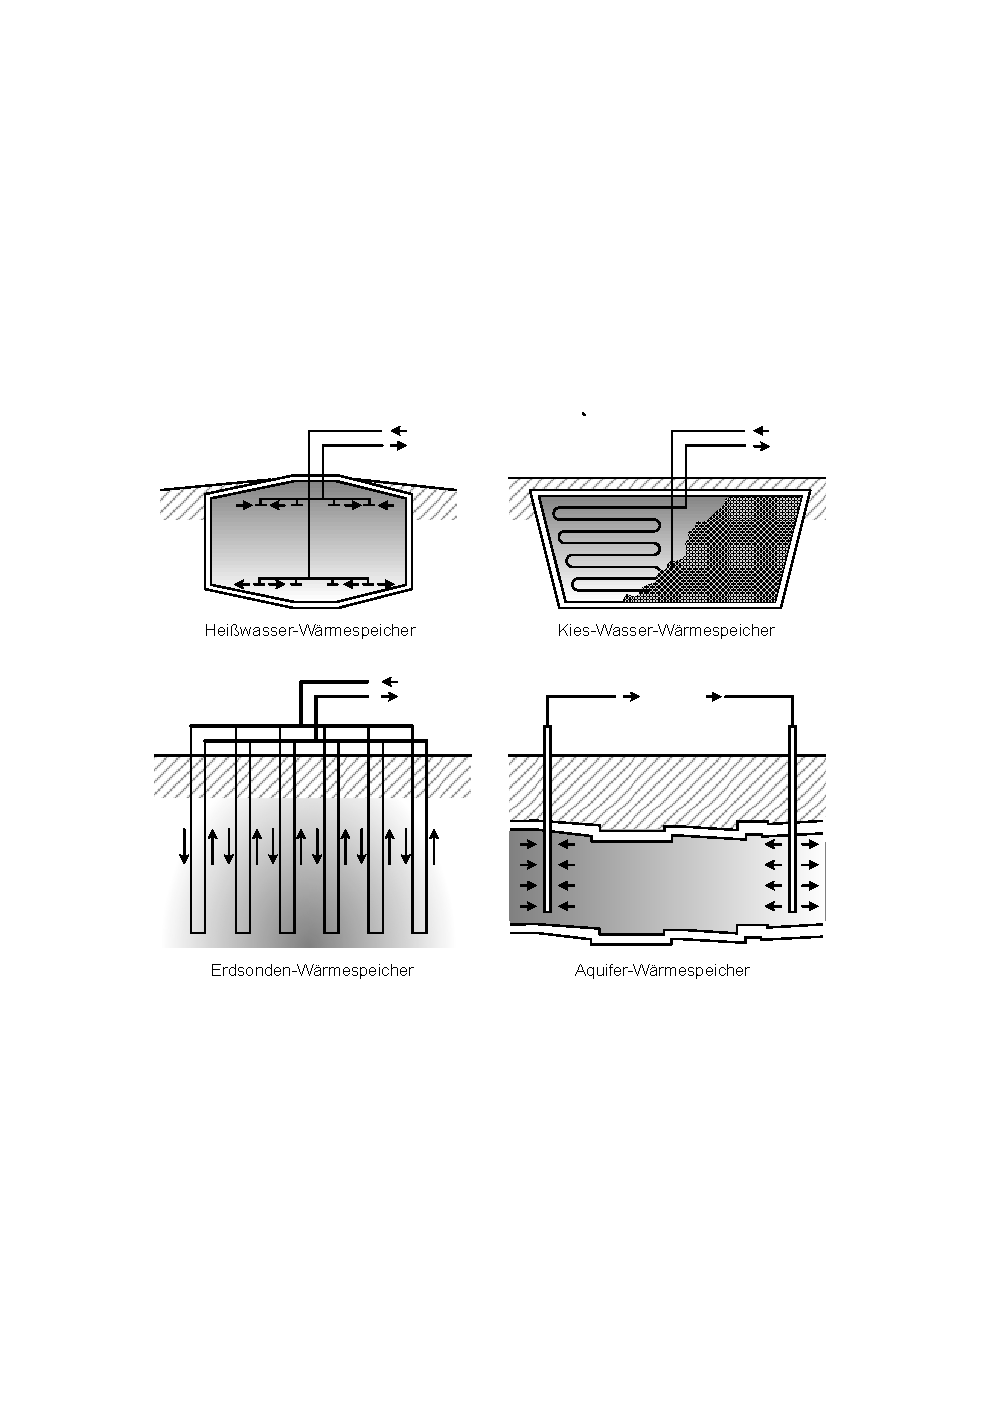
\includegraphics[scale=1]{images/langzeitspeicher.pdf}
\caption{Langzeitsensibelwärmespeicher \cite{Wesselak}}
\label{fig:Langzeitspeicher}
\end{center}
\end{figure}

\section{Technologischer Überblick}
In diesem Kapitel werden der Stand der Technik, die Entwicklung, Perspektiven
und Herausforderungen der zwei zu behandelnden Speichertechnologien erläutert.
\subsection{Latentspeicher}
In den folgenden Unterkapiteln wird ein allgemeiner Überblick über
Latentwärmespeicher gegeben und danach spezifisch auf den Stand der Technik und
die zukünftige Entwicklung eingegangen.
\subsubsection{Allgemein}
Latentspeicher nützen den Phasenwechsel aus. Jedes Material besitzt einen
sogenannten Schmelz- bzw. Erstarrungspunkt und einen Siede- bzw.
Kondensationspunkt. An diesem Temperaturpunkt wechselt das Medium sine Phase von
fest zu flüssig bzw. von flüssig zu gasförmig. Um diese Phasenänderung
vorzunehmen benötigt das Medium viel Wärmeenergie bzw. gibt viel Wärmeenergie an
die Umgebung ab. Das Beispiel in Abbildung \ref{fig:H2O} zeigt die Benötigte
Wärmeenergie für die Temperaturerhöhung und den Phasenübergang von Wasser bei
Normdruck auf.

\begin{figure}[h!]
\begin{center}
\includegraphics[scale=0.6]{images/Phasendiagramm.pdf}
\caption{Phasenübergänge von \ce{H_2O} und die dafür benötigten Energiemengen}
\label{fig:H2O}
\end{center}
\end{figure}
Deutlich zu erkennen ist einerseits die enorm grosse Schmelz- und
Verdampfungswärme im Vergleich zu der temperaturerhöhenden Wärme. Zu
berücksichtigen ist dabei, dass die X-Achse nicht linear verläuft. Andererseits
ist ersichtlich, dass die zum Phasenwechsel benötigte Wärme auf demselben
Temperaturniveau stattfindet. Die Schmelz- und Verdampfungswärme wird auch als
latente Wärme bezeichnet. Die restliche Wärme, welche eine Temperaturdifferenz
hervorruft wird sensible Wärme genannt.
Der Temperaturpunkt, an welchem der Phasenübergang stattfindet ist vom Medium
und vom herrschenden Druck abhängig. Abbildung \ref{fig:H2O2} zeigt das
Phasendiagramm von Wasser. Erkennbar ist, dass der Schmelz- und Siedepunkt sich
mit Veränderung des Druckes ebenfalls ändern
\begin{figure}[h!]
\begin{center}
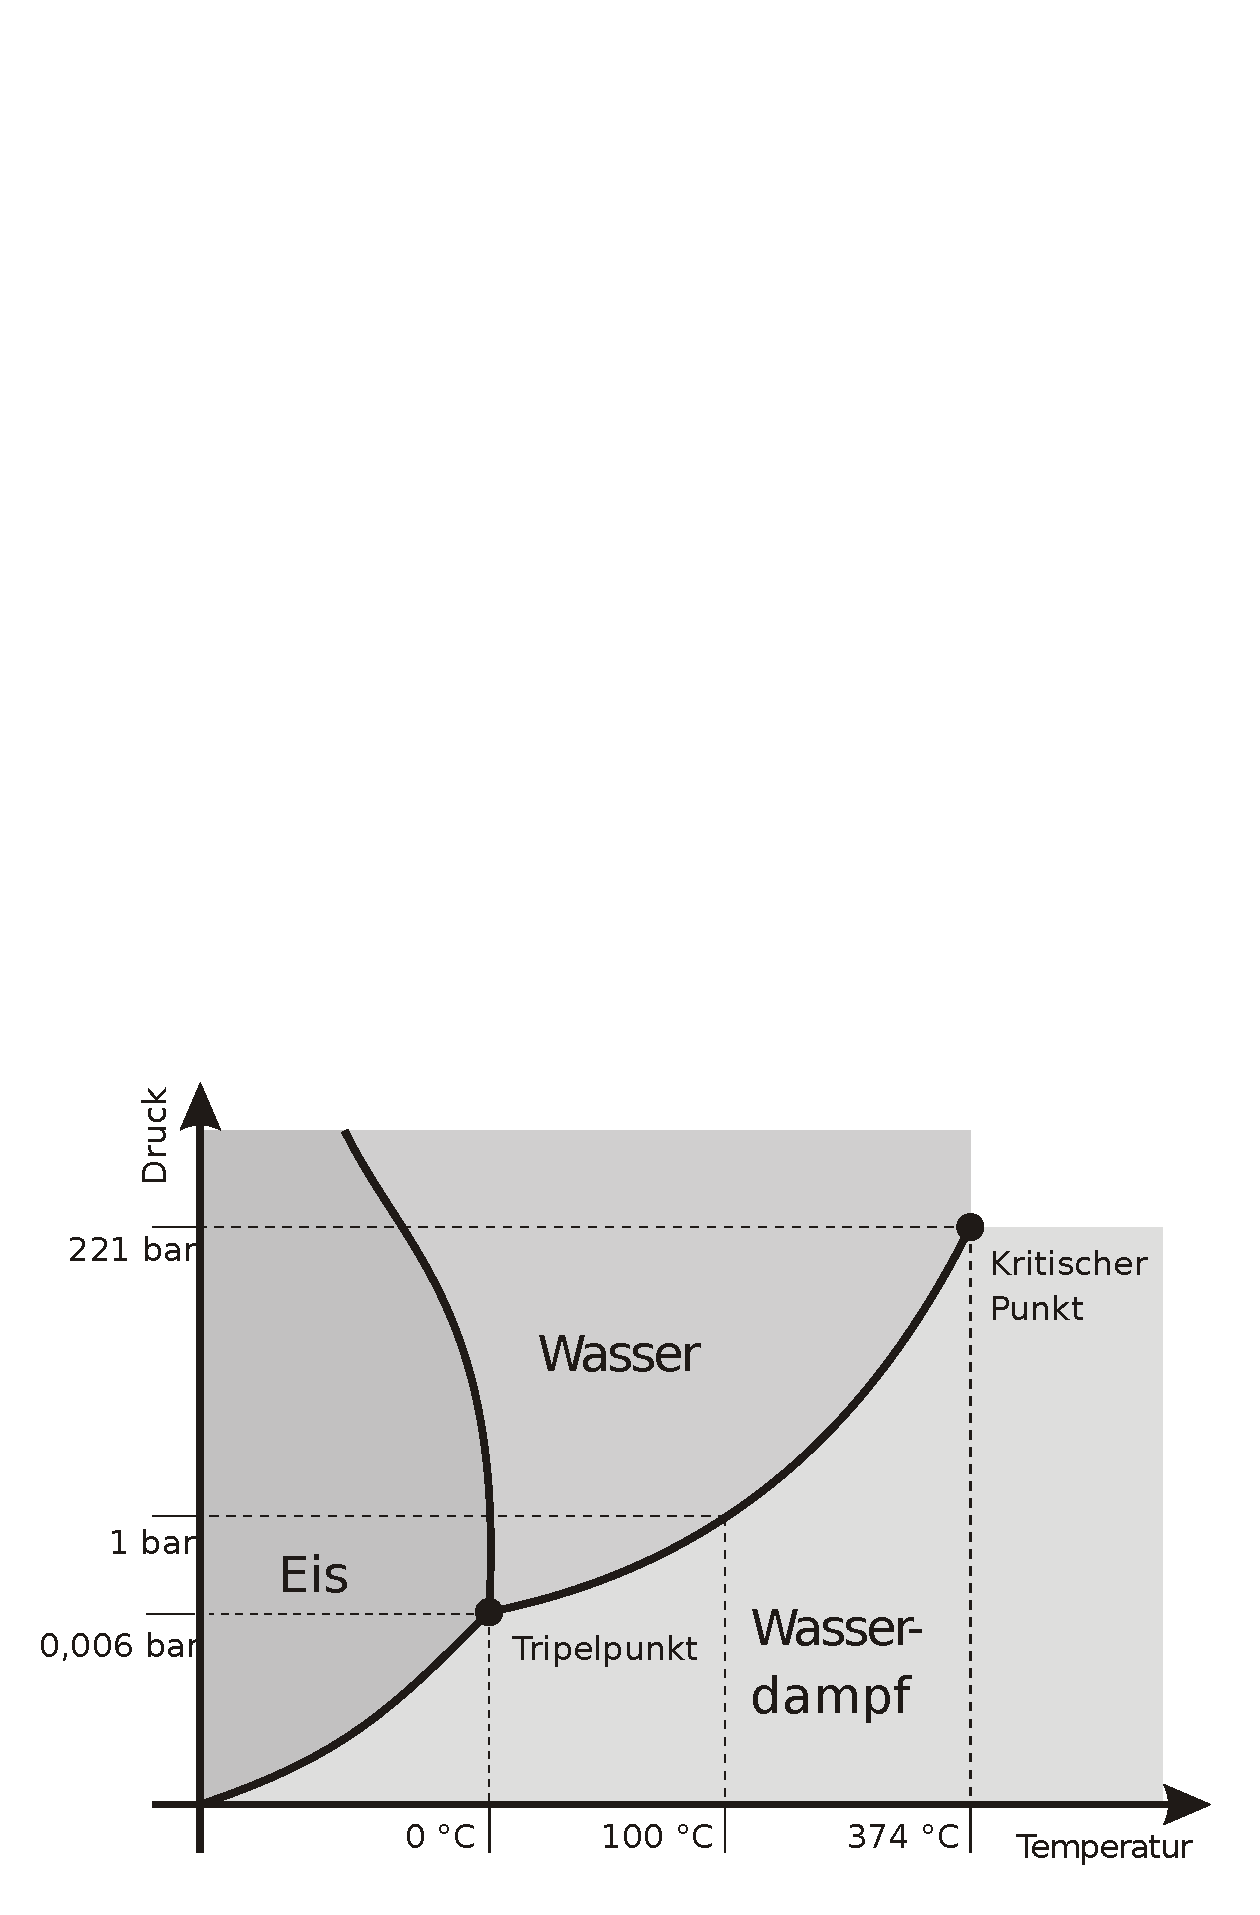
\includegraphics[scale=0.6]{images/Phasendiagramm2d.pdf}
\caption{Phasendiagramm von \ce{H_2O} \cite{Phasendiagramm}}
\label{fig:H2O2}
\end{center}
\end{figure}
Bei einem Latentwärmespeicher versucht man somit ein Medium unter einem gewissen
Druck zu halten, damit dieses einen Phasenwechsel vornimmt bei einer gewünschten
Temperatur. Dadurch kann viel Energie bei keinem Temperaturhub gespeichert
werden. Mit der untenstehenden Formel lässt sich die speicherbare Energie
einfach berechnen:

\begin{align}
\Delta Qv = m \cdot (\Delta U + p \cdot \Delta V) = m \cdot \Delta Hv
\label{eq:latent}
\end{align}

\begin{table}[h!]
\begin{center}
\begin{tabular}{|l|p{5cm}|l|}
\hline $\Delta Qv$ & Schmelz- bzw. Verdampfungswärme & [J] \\
\hline $m$ & Masse & [kg] bzw [mol] \\
\hline $\Delta Hv$ & Spezifische Schmelz- bzw. Verdampfungsentalphie & [J/kg]
bzw. [J/mol] \\
\hline
\end{tabular}
\caption{Variablen der Gleichung \ref{eq:latent}}
\end{center}
\end{table}

Dabei hängt die Masse von der Grösse des Speichers ab und die spezifische
Enthalpie ist Mediumsabhängig.


\subsubsection{Stand der Technik}
Im Gegensatz zu sensiblen Wärmespeicher, werden Latentwärmespeicher weniger
häufig eingesetzt. Wie Tabelle \ref{tab:Wesselak1} zeigt sind verschiedene
Latentspeicher entwickelt aber noch nicht ausgereift.

\begin{table}[h]
\begin{center}
\caption{Speicherkapazität und Entwicklungsstand thermischer Speicher
\cite{Wesselak} S.682}
\label{tab:Wesselak1}
\begin{tabular}{@{}lp{2cm}p{3cm}p{2.7cm}l@{}}
\toprule
                  Speicherart & Stoff & Arbeitstemperatur \newline[$^{\circ}
                  C$]& Speicherkapazität \newline [kWh/m$^3$] &
                  Entwicklung
                  \\
                  \toprule \multirow{2}{*}{Sensibel} & Wasser  & 0-100 & 60 &
                  ausgereift
                  \\
                  & Beton & 0-500 & 30 & ausgereift  \\ \hline
\multirow{3}{*}{Latent} &Paraffine  & 0-70 & 60  & entwickelt  \\
                  & Salzhydrate & 30-100 & 150 & entwickelt \\
                  & Salze  & 100-400 & 100 & entwickelt \\ \hline
\multirow{3}{*}{Thermochemisch} & Silikagele & 40-100 & 200 & in Entwicklung  \\
                  & Zeolithe & 100-300  & 200 & in Entwicklung \\
                  & Metallhydride & 300-900 & 500 & in Entwicklung  \\ \toprule
\end{tabular}
\end{center}
\end{table}
Bei der Entwicklung von Latentwärmespeicher geht es vorwiegend um die
Herstellung eines optimalen Speichermediums. Dieses muss neben der möglichst
hohen spezifischen Phasenumwandlungsenthalpie noch viele weitere Kriterien
einhalten. Einige Anforderungen sind gemäss \cite{Wesselak} die folgenden:
\begin{itemize}
  \item Die Phasenwechseltemperatur muss im geforderten Arbeitsbereich liegen.
 \item Der Stoff sollte eine möglichst hohe spezifische
  Phasenumwandlungsenthalpie haben, damit je Masseeinheit des Speicherstoffes eine möglichst grosse
Wärmemenge gespeichert wird.
\item Der Stoff sollte eine möglichst hohe Dichte haben, um ein hohes
volumenbezogenes Speichervermögen aufzuweisen.
\item Der Stoff sollte eine hohe spezifische Wärmekapazität haben, da in der Regel
Energie auch als sensible Wärme gespeichert wird.
\item Der Stoff sollte eine möglichst hohe Wärmeleitfähigkeit besitzen, damit eine
Wärmeübertragung schon bei kleinen Temperaturdifferenzen mit relevanten
Leistungen möglich ist.
\item Der Stoff sollte ein kongruentes Schmelzverhalten haben und ohne feste
Zwischenphasen direkt aus dem festen Zustand in die homogene Schmelze übergehen
und umgekehrt. Andernfalls könnte es im Verlauf eines oder mehrerer Zyklen zu
Entmischungen und einer Abnahme der Wärmespeicherkapazität kommen.
\item Der Stoff sollte eine möglichst kleine Volumenänderung beim Phasenwechsel
aufweisen, um die mechanischen Belastungen für Speicherraum und Peripherie
möglichst gering zu halten.
\item Der Stoff sollte nicht zu Unterkühlungen neigen.
\item Der Stoff sollte chemisch und physikalisch in dem geforderten
Temperaturbereich langzeitstabil sein.
\item Der Stoff sollte keinen eng zusammen liegenden Schmelz- und Siedepunkt haben,
damit es nicht zur Verdampfung bei einer möglichen Überhitzung über den
Schmelzpunkt hinaus kommen kann.
\item Der Stoff sollte nicht korrosiv auf die verwendeten Konstruktionsmaterialien
wirken.
\item  Der Stoff darf weder toxisch, noch entflammbar oder explosiv sein. Hinzu
kommen ökonomische und ökologische Anforderungen wie die Verfügbarkeit in
grossen Mengen, ein möglichst niedrigerer Preis, Umweltverträglichkeit,
Recyclingfähigkeit und Wiederverwendbarkeit nach Erreichen der Nutzungsdauer des
Wärmespeichers.
\end{itemize}
Viele Medien befinden sich heutzutage noch in der Entwicklung. Für den
Gebäudebereich, wo häufig eine Speichertemperatur von ca. 65°C erwünscht ist,
ist das Speichermedium Natriumhydroxid-Monohydrat (\ce{NaOH - H_2O}) das
beliebteste Medium. Es weist für diesen Temperaturbereich die günstigsten
Gesamteigenschaften auf und ist bereits gut erforscht. Auch andere
Speichermedien sind bereits erforscht, haben jedoch teilweise andere
Eigenschaften und Schmelzpunkte beim selben Druck. Einige davon sind in Tabelle
\ref{tab:salz} aufgelistet.

\begin{table}[h!]
\begin{center}
\caption{Vergleich von Speichersalzsystemen für den Temperaturbereich von 0-100
$^\circ$C \cite{Wesselak}}
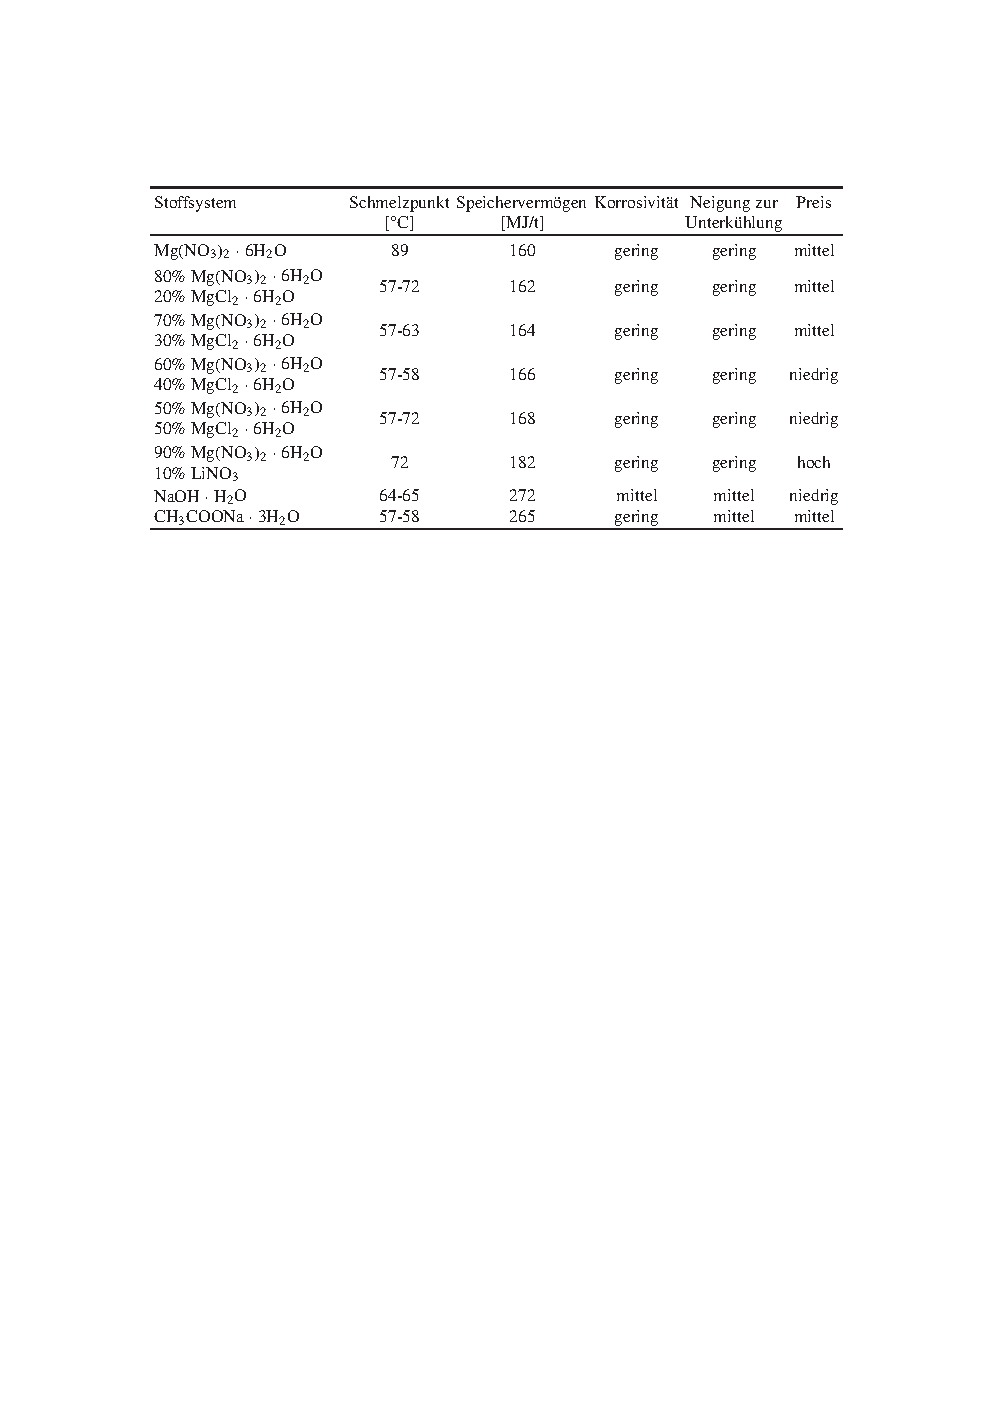
\includegraphics[scale=1]{images/speichersalze.pdf}
\label{tab:salz}
\end{center}
\end{table}
Die Hauptprobleme, welche man mit Forschungs- und Entwicklungsprojekte beheben
möchte, sind einerseits die schlechte Leitfähigkeit von Phase Change Material
(PCM). Andererseits ist es die Unterkühlung der Salzhydrate. Unterkühlung
bedeutet, dass der Phasenwechsel von Flüssig zu Fest erst bei einer zu tiefen
Temperatur stattfindet und somit eine thermodynamische Entwertung der
gespeicherten Energie vorliegt. Das erstgenannte Problem versucht man durch eine
Verkapselung und somit Vergrösserung der Oberfläche zu lösen. Den erwähnten
Unterkühlungseffekt versucht man durch das Zusetzen von Keimbildnern zu
verhindern.

Forschung wird ebenfalls betrieben um die Speicherkapazität von Gebäuden zu
erhöhen. Dies ist derzeit das grösste Einsatzfeld von PCM. Dafür wird  PCM in
die Baustoffe integriert. Solche Materialien sind heutzutage bereits kommerziell
erhältlich und werden eingesetzt.


\subsubsection{Entwicklung und Perspektiven}
Bis heute ist es noch nicht gelungen, Salzhydrate in Mikrokapseln einzubinden.
Dies versucht man jedoch in Zukunft zu ändern, um die Vorteile von Salzhydraten
gegenüber Paraffinen auszunutzen. Diese sind höhere Schmelzenthalpie und
Unentflammbarkeit. Weiter sollen durch Forschungsprojekte die Materialkosten
gesenkt und die Energiedichten erhöht werden. Die heutzutage noch fehlende
Langzeiterfahrung und die erhöhten Kosten zur Effizienzsteigerung im Gegensatz
zu sensiblen Wärmespeicher im Gebäudeeinsatz lässt die Wirtschaftlichkeit von
latenten Wärmespeichern in Frage stellen. Verschiedene Forschungsprojekte
möchten jedoch einen wirtschaftlichen Vorteil gegenüber sensiblen Speichern
erreichen.

\subsection{PCM Slurries}
In diesem Kapitel werden thermodynamische Eigenschaften von PCM-Slurries
aufgezeigt und mit denen von Wasser verglichen.
\subsubsection{Thermodynamischer Sachverhalt}
Heutzutage werden die meisten Gebäude mit einem Wassersystem geheizt und
gekühlt. Wasser wird aus verschiedenen Gründen verwendet. Grosse Vorteile sind
dabei die hohe spezifische Wärmekapazität, die Umweltverträglichkeit und der
günstige Preis. Wasser hat beispielsweise pro Kilogramm eine viermal höhere
Wärmekapazität als Luft. Somit lässt sich dieselbe Energie mit einem deutlich
kleineren Massenstrom befördern. Mit der folgenden Formel kann die Abhängigkeit
zwischen Medium, Massenstrom, Temperaturänderung und Wärmetransport aufgezeigt
werden.

\begin{align}
\dot{Q}=\dot{m} \cdot c_p \cdot \Delta T
\label{eq:PCM}
\end{align}

\begin{table}[h!]
\begin{center}
\caption{Variablen der Gleichung \ref{eq:PCM}}
\begin{tabular}{|l|l|l|}
\hline $\dot{Q}$ & Wärmeleistung & [W] \\
\hline $\dot{m}$ & Massenstrom & [kg/s] \\
\hline $c_p$ & spezifische Wärmekapazität & [J/kg $\cdot$ K] \\
\hline $\Delta T$ & Temperaturdifferenz zwischen Vor- und Rücklauf & [K] \\
\hline
\end{tabular}
\end{center}
\end{table}
Die spezifische Wärmekapazität hängt dabei vom entsprechenden Medium ab. Je
höher der Massenstrom bei gleichbleibender Wärmeleistung umso geringer die
Temperaturdifferenz. Um einen optimalen Betrieb des Heizungs- bzw. Kühlsystems
zu erreichen sollte einerseits die Temperatur des Mediums möglichst tief gewählt
werden um Wärmeverluste zu minimieren und allenfalls der Coefficient of
Performance (COP) der Wärmepumpe bzw. Kältemaschine zu erhöhen. Andererseits
sollte auch der benötigte Strom für die Beförderung des Mediums möglichst gering
gehalten werden. Dies erhält man mit einem möglichst kleinen Massenstrom. Es
liegt ein Optimierungsproblem vor.

\subsubsection{Vergleich Viskosität und Energiedichte}
Um sowohl den Massenstrom bzw. Beförderungsantriebsleistung, wie auch die
Temperaturdifferenz kleiner zu machen, müssen die Mediumseigenschaften
verbessert werden. Dies versucht man mit Hilfe von PCM – Slurries (PCS). Dies
sind Fluide, welche aus verkapseltem PCM bestehen, gemischt mit Wasser. Da die
latente Wärme anstelle der sensiblen genutzt wird, wird eine sehr geringe
Temperaturdifferenz benötigt und die Energiedichte steigt enorm an.
Abbildung \ref{fig:PCSWasser} zeigt die spezifische Enthalpie im Vergleich zu
Wasser bei unterschiedlichem Schmelzbereich und PCS-Konzentration.

\begin{figure}[h!]
\begin{center}
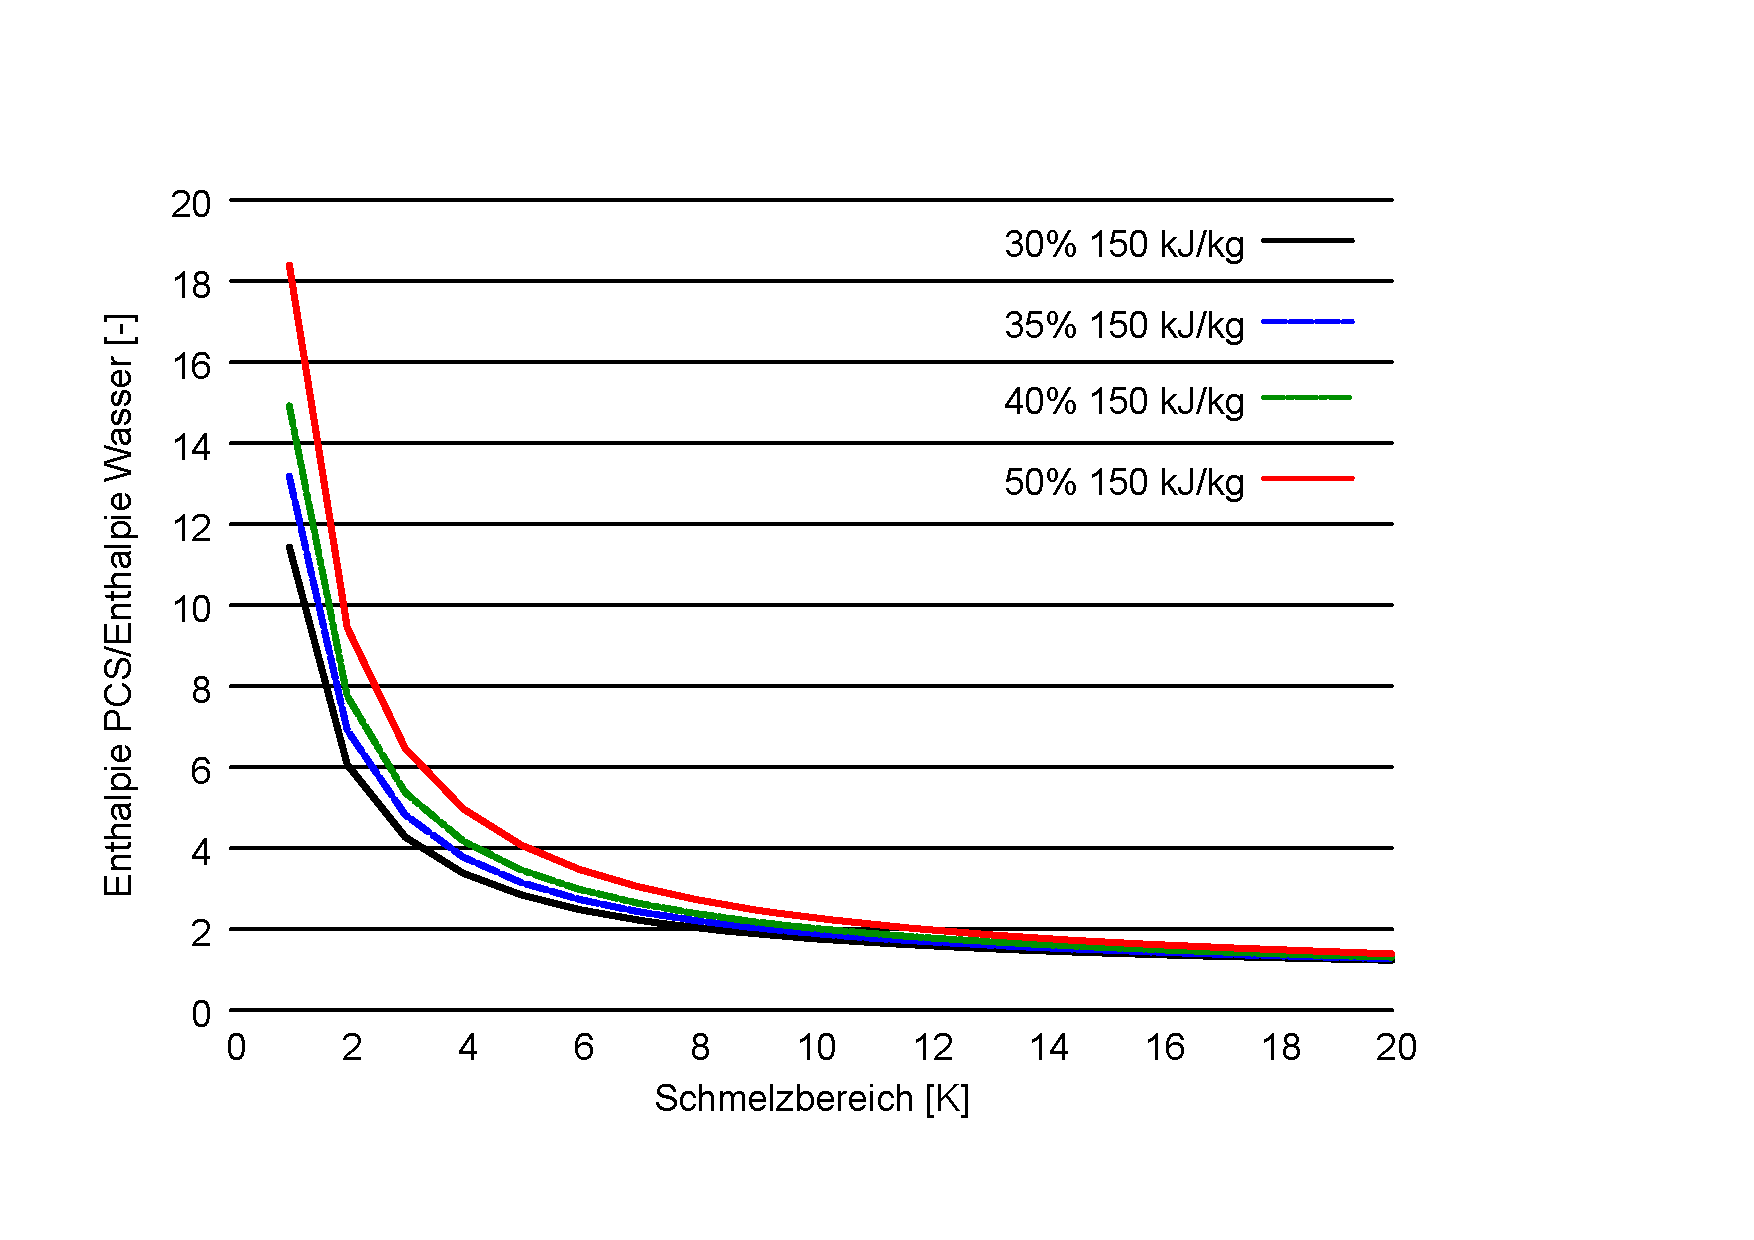
\includegraphics[scale=0.4]{images/Henning1.pdf}
\caption{Enthalpie von PCS im Vergleich mit Wasser \cite{Henning}}
\label{fig:PCSWasser}
\end{center}
\end{figure}
Je nach Viskosität sind heutzutage Mischungen bis zu 50\% möglich. Leider ist
die Viskosität von PCS schlechter als jene von Wasser und es entsteht dadurch
ein erhöhter Energiebedarf für Pumpen. Abbildung \ref{fig:PCSDruck} zeigt den
Druckverlust einer 30\% Emulsion im Vergleich zu Wasser auf. Vergleicht man dies
jedoch wieder mit der erhöhten Enthalpie der PCS kann mit PCS bei gleicher
Pumpenleistung deutlich mehr Wärmeenergie transportiert werden
\begin{figure}[h!]
\begin{center}
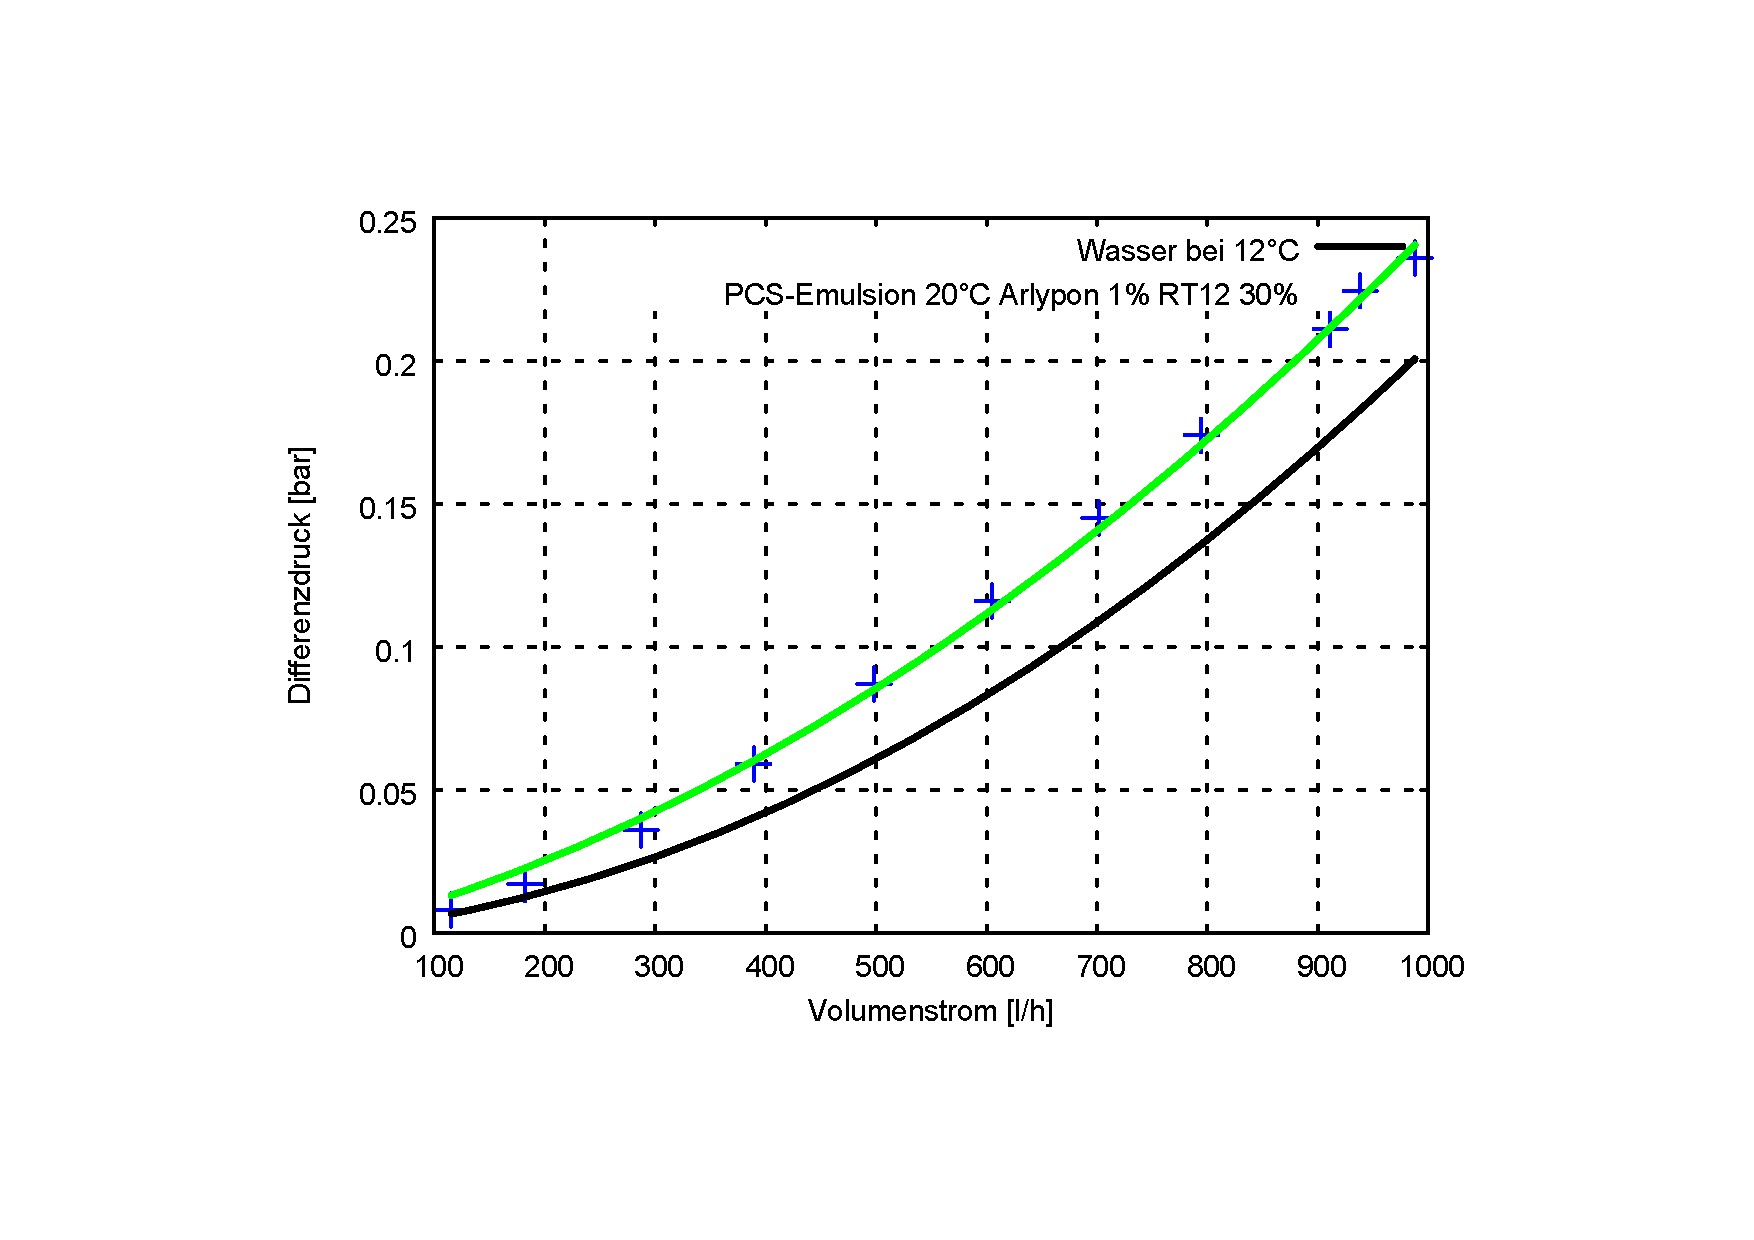
\includegraphics[scale=0.4]{images/Henning2.pdf}
\caption{Druckverlust von PCS im Vergleich zu Wasser \cite{Henning}}
\label{fig:PCSDruck}
\end{center}
\end{figure}
Dies liegt an den thermodynamischen Eigenschaften, welche sich je nach
Konzentration verändern. Tabelle \ref{tab:PCSThermo} zeigt diese Veränderung auf
für PCS bis zu 20\%.

\begin{table}[h!]
\begin{center}
\caption{Thermodynamische Eigenschaften von PCS \cite{Gschwander}}
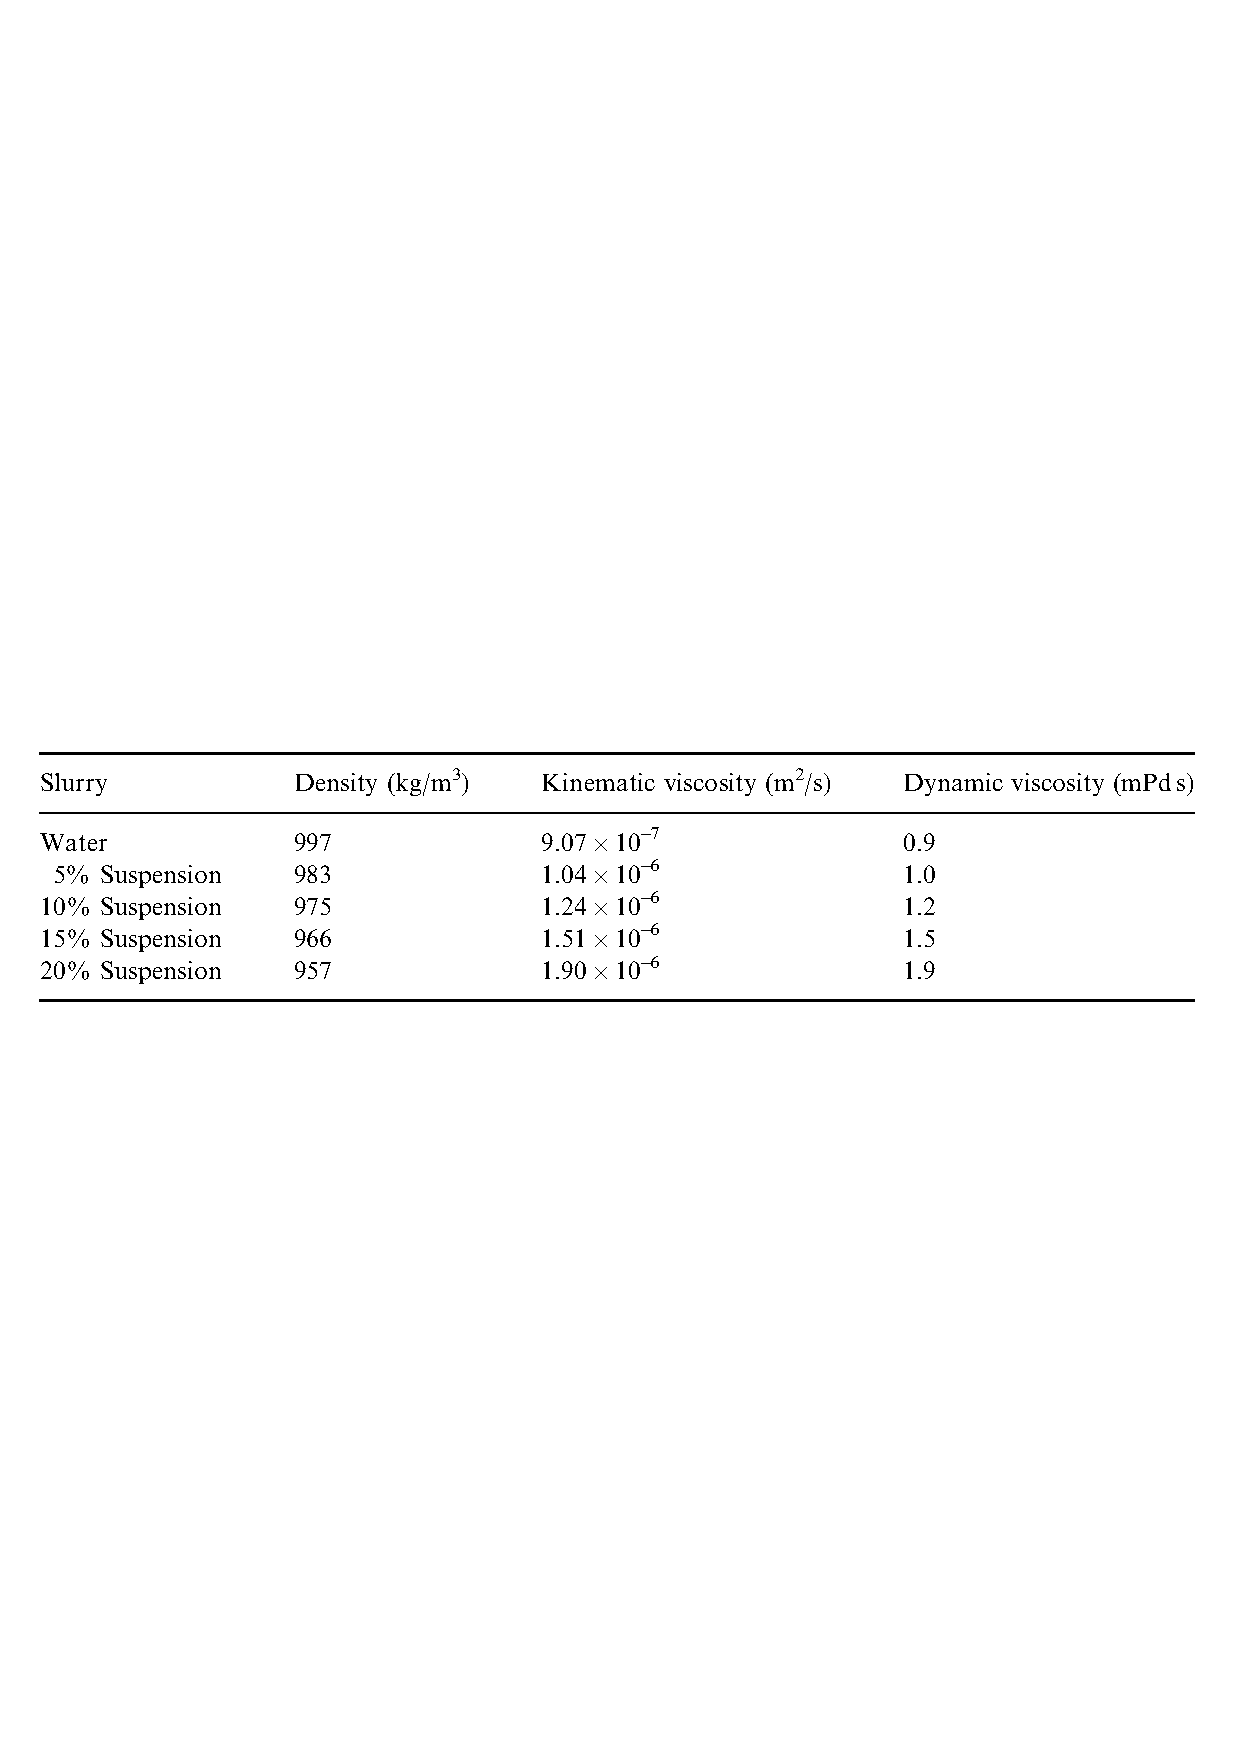
\includegraphics[scale=0.6]{images/HenningTable.pdf}
\label{tab:PCSThermo}
\end{center}
\end{table}

Grafik \ref{fig:BINEVisko} zeigt auf einen Blick die Speicherkapazität und die
Viskosität im Vergleich zu Wasser. Somit stellt sie den oben diskutierten
Sachverhalt nochmals zusammenfassend dar.
\begin{figure}[h!]
\begin{center}
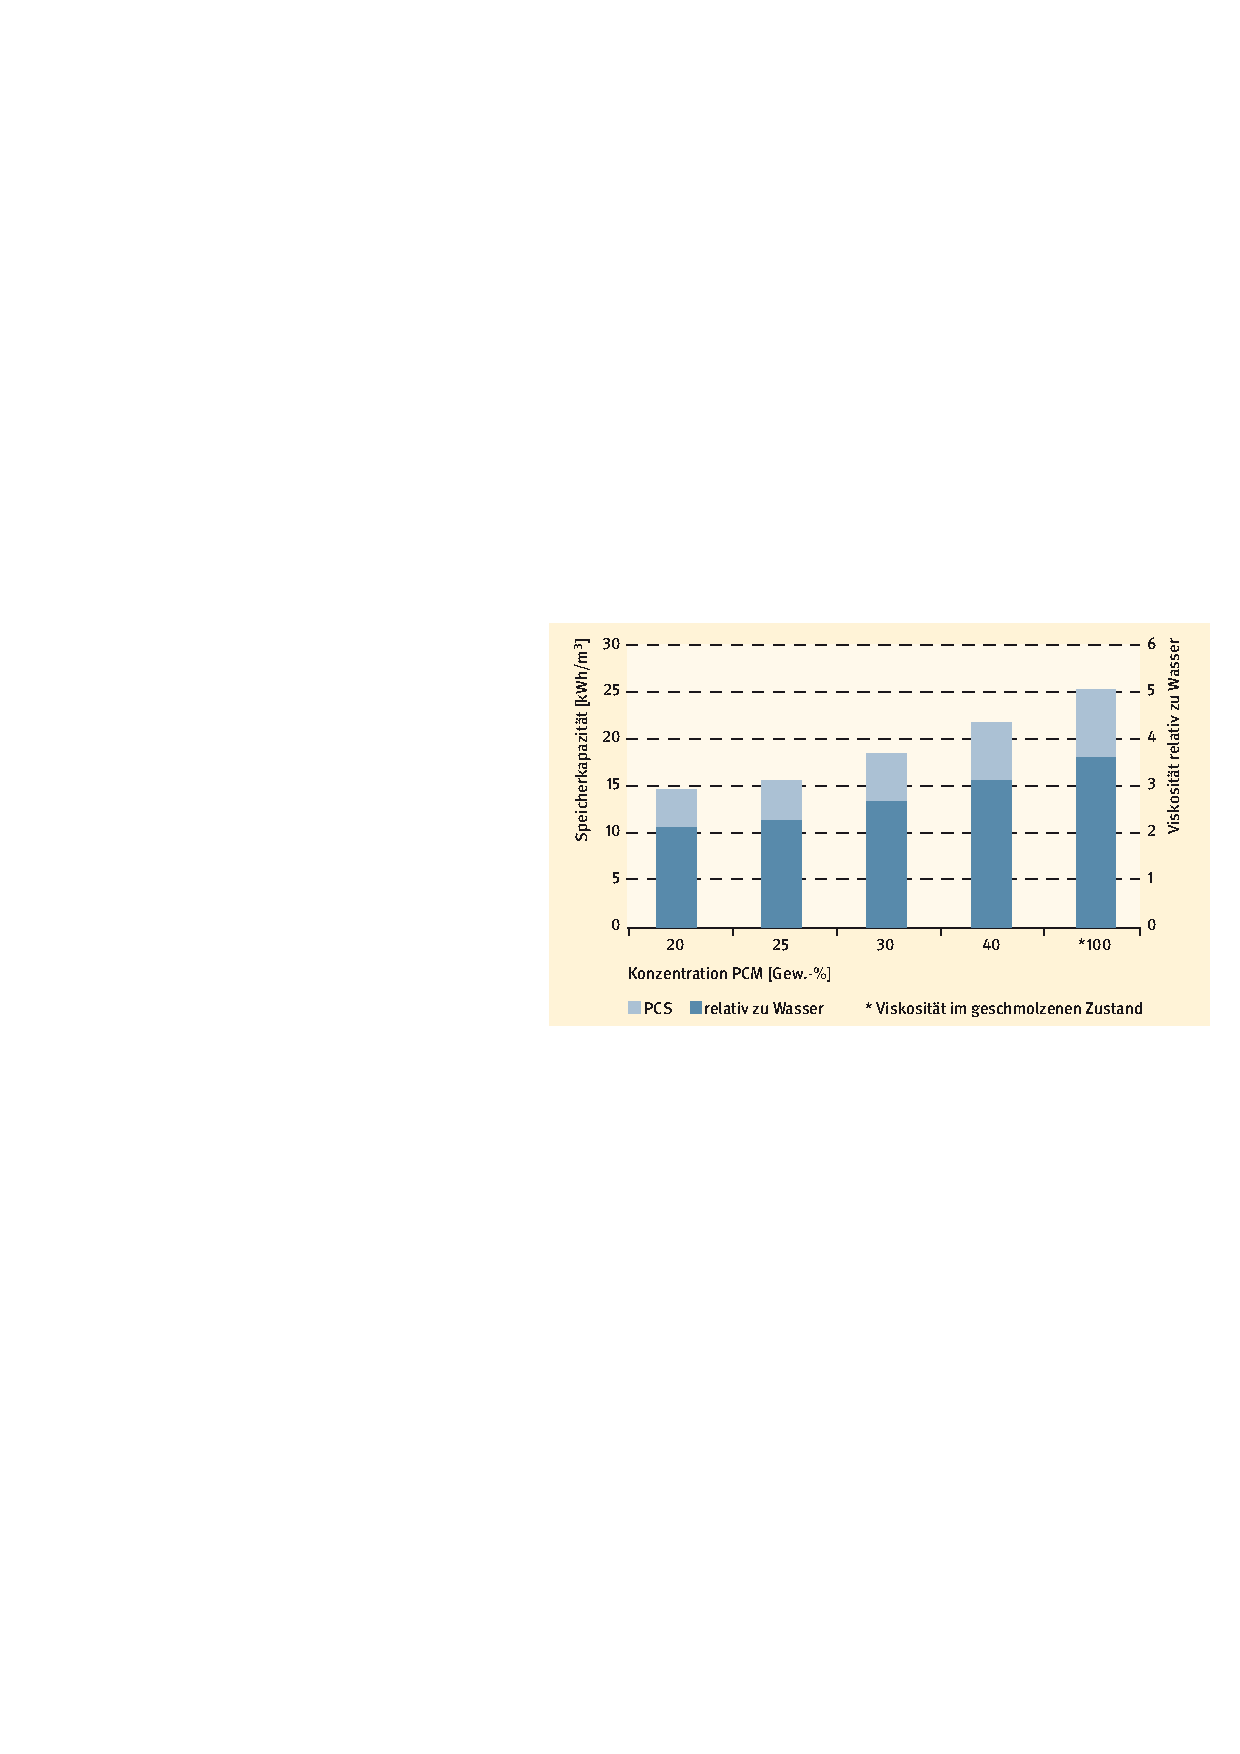
\includegraphics[scale=0.8]{images/BineVisko.pdf}
\caption{Speicherkapazität und Viskosität von PCS im Vergleich zu Wasser
\cite{BINE3}}
\label{fig:BINEVisko}
\end{center}
\end{figure}
\subsubsection{Vergleich Temperaturdifferenz}
Ein weiterer Vorteil, welcher durch die geringe Temperaturdifferenz von PCS
entsteht ist die Erhöhung der Jahresarbeitszahl von Wärmepumpen bzw.
Kältemaschinen durch die tieferen erforderlichen Temperaturen. Vor allem in der
Übergangszeit ist es, mit solchen Fluiden, länger möglich, mit dem
Freecoolingbetrieb das Gebäude zu kühlen. Es ist somit erwünscht, dass das
Medium eine möglichst hohe Enthalpiedifferenz bei möglichst geringer
Temperaturerhöhung erreicht. In Abbildung \ref{fig:GschwanderEnt} ist ein solcher
Vergleich vorhanden. Der Phasenwechsel findet bei diesem Beispiel zwischen 23
und 27°C statt. Die Temperaturdifferenz ganz zu eliminieren ist zurzeit noch
nicht möglich.
\begin{figure}[h!]
\begin{center}
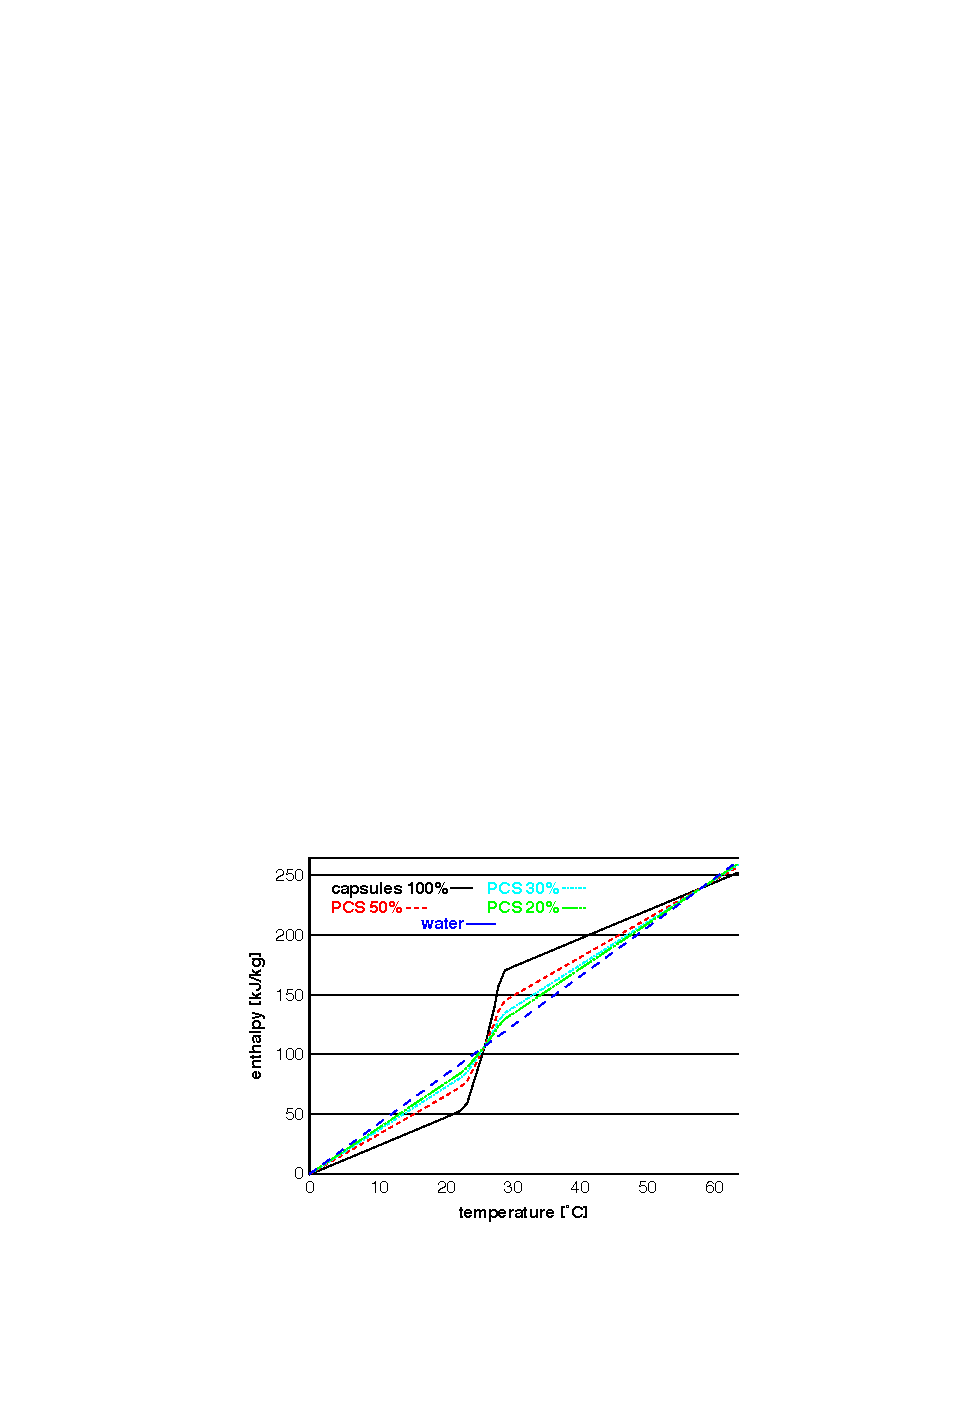
\includegraphics[scale=1]{images/GschwanderEnt.pdf}
\caption{Vergleich zwischen Enthalpie und Temperatur \cite{Gschwander}}
\label{fig:GschwanderEnt}
\end{center}
\end{figure}

\subsubsection{Herausforderungen}

Die Phase Change Material, PCM nutzen den Phasenwechsel aus was zu neuen Herausforderungen führt. Der Aggregatszustandswechsel zwischen fest und flüssig wie auch der Wechsel von flüssig zu gasförmig hat seine Eigenheiten. Konstruktiv ist bei dem Phasensenwechsel zwischen fest und flüssig eine Herausforderung die Wärme im Raum zu verteilen, dies wird nachfolgend genauer beschrieben. Anderseits ist beim übergang von flüssig zu gasförmig die Herausforderung der ganz verschiedenen Dichten und somit Volumen ein Problem.

Wir uns anhand eines Experiments den Schmelzprozess im Raum genauer an. Dabei handelt es sich um einen kugelförmigen Raum, darin befindet sich ein PCM-Werkstoff, welches zu Beginn überall als Festkörper besteht. Die Kugelform befindet sich in einem Wasserbad, wodurch es möglich ist eine konstante Temperatur der Kugeloberfläche zu bekommen. In der Abbildung \ref{fig:meltingpaper} (a) ist ein sogenanntes Ungezwungenes System, und die Abbildung \ref{fig:meltingpaper} (b) zeigt ein eingeschränktes System, dies bedeutet in diesem Fall, es hat ein vertikales Rohr, wo Thermoelemente darin befinden sich.

\begin{figure}[h!]
\begin{center}
% Dieses Bild sollte erstezt werden
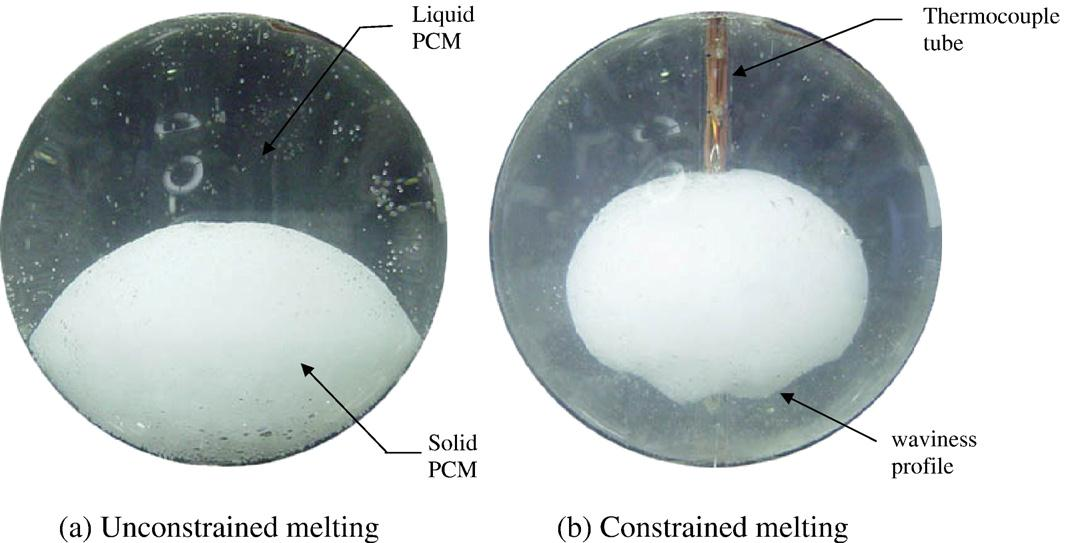
\includegraphics[scale=0.4]{images/Meltinginsidesphere.jpg}
\caption{Schmelzprozess innerhalb einer Kuge. a) nicht konstantes schmelzen und b) konstantes Schmelzen \cite{WasteEnergyHarvesting}}
\label{fig:meltingpaper}
\end{center}
\end{figure}

Wird das Experiment nun gestartet ergeben sich zwei unterschiedliche Formen und auch die Zeit bis das ganze PCM geschmolzen ist verhält sich nicht gleich. In der Abbildung \ref{fig:meltingphasefront} ist dargestellt wie das verhalten über der Zeit ist. Es ist zu erkennen, das der Fall des eingeschränkten System etwa ein Drittel länger braucht als das ungezwungene System bis das PCM total flüssig ist. Dies ist auf den ersten Blick wohl eher verwunderlich.

\begin{figure}[h!]
\begin{center}
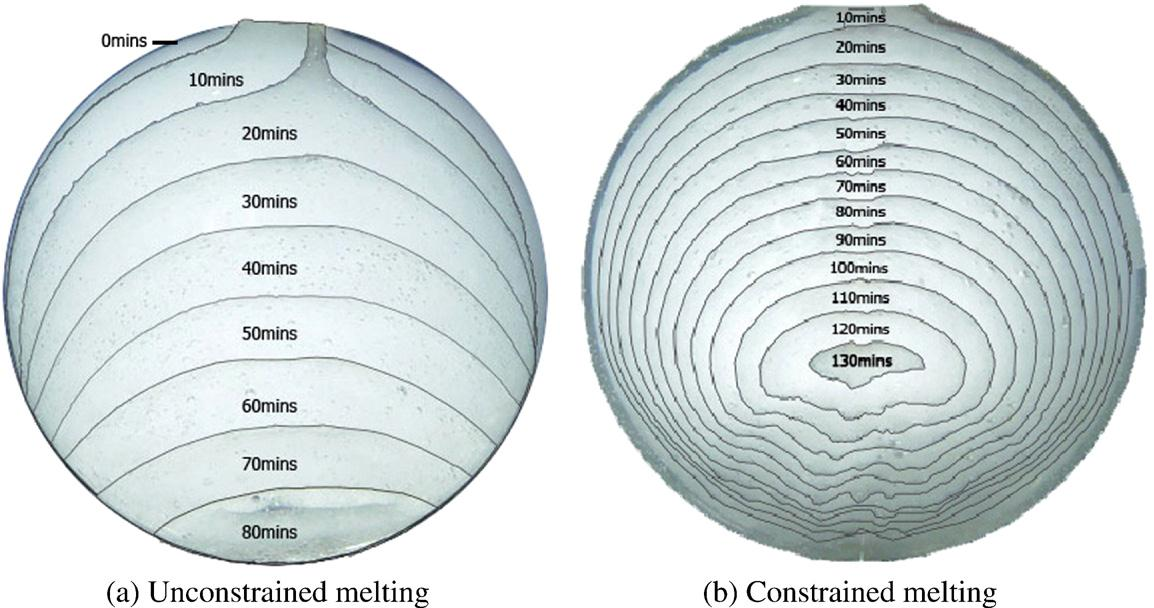
\includegraphics[scale=0.35]{images/meltingphasefront.jpg}
\caption{Serie der Schmelzfront über bei verschiedenen Zeitpunkten \cite{meltingpaper}}
\label{fig:meltingphasefront}
\end{center}
\end{figure}

Nun betrachten wir die Gründe, weshalb ein ungezwungene Schmelzung in diesem
Fall schneller von statten geht als das gezwungene System. Die Abbildung
\ref{fig:heatconductionin} zeigt die natürliche Konvektion, des ungezwungenen
und des eingeschränkten Experiment. Die natürliche Konvektion, also die durch
den Dichteunterschied und Gravitationskraft getriebener Austausch und die
Wärmeleitfähigkeit spielen dabei eine wesentliche Rolle. Bei der eingeschränkten
Experiment mit dem Rohr in der Mitte beginnt es gleichmässig von aussen nach
innen zu schmelzen, dies funktioniert zu Beginn auch optimal, da der
Phasenwechsel direkt an der Kugelaussenwand passiert. Schon nach kurzer Zeit
grenzt keine Festphase mehr an die Aussenwand und es stellt sich eine natürliche
Konvektion ein siehe Abbildung \ref{fig:heatconductionin} (b) welche rings um
den Festkörper wirkt und so eine Barriere wirkt für den Phasenwechsel. Bei dem
Experimentfall beginnt es langsamer geht dann schlussendlich schneller bis das
ganze PCM geschmolzen ist. Dies ist so, weil dauernd der Kontakt der festen
Phase mit der Kugeloberfläche besteht und dieser Effekt durch das Eigengewicht
der festen Phase immer besteht.

\begin{figure}[h!]
\begin{center}
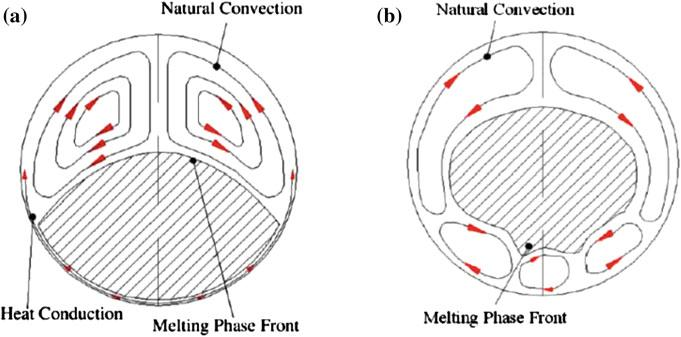
\includegraphics[scale=0.6]{images/heatconductionin.jpg}
\caption{Wärmeleitung und natürliche konvektion in nicht konstantem Fall a) und im konstanten Fall b) \cite{WasteEnergyHarvesting}}
\label{fig:heatconductionin}
\end{center}
\end{figure}

Der Vergleich zeigt, dass in diesem Untersuchen Fall, als das Schmelzen eines kugelförmigen PCM besser keine einbauten hat, da die natürlichen Effekte ein schlussendlich schnelleres schmelzen verursachen.

Es gibt auch andere Überlegungen von der Anordnung und Form für das PCM. So zum Beispiel mit Rippen, siehe Abbildung \ref{fig:threedimensionalphysicalmodel} und auch hier gibt es gewünschte und ungewünschte Effekte wie Experimente und Simulationen zeigen. Aber auch Zylinder mit verschiedensten Arten von Material das eine gute Leitfähigkeit hat und nicht viel Volumen benötigt und dies zum Teil strukturiert oder unstrukturiert verteilt, siehe Abbildung \ref{fig:simulatedvelocity}

\begin{figure}[h!]
\begin{center}
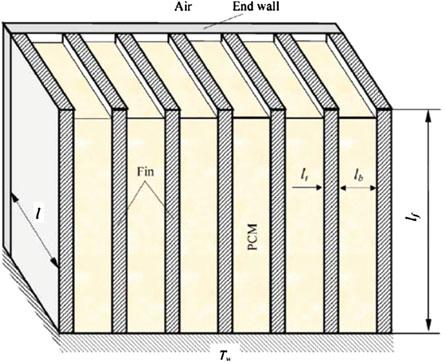
\includegraphics[scale=0.4]{images/threedimensionalphysicalmodel.jpg}
\hspace{1cm}
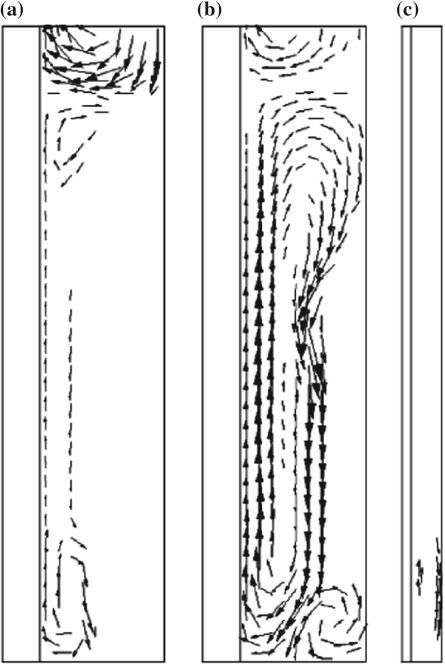
\includegraphics[scale=0.2]{images/simulatedvelocity.jpg}
\caption{Vergleich zwischen Enthalpie und Temperatur \cite{WasteEnergyHarvesting}}
\label{fig:threedimensionalphysicalmodel}
\label{fig:simulatedvelocity}
\end{center}
\end{figure}


\begin{figure}[h!]
\begin{center}
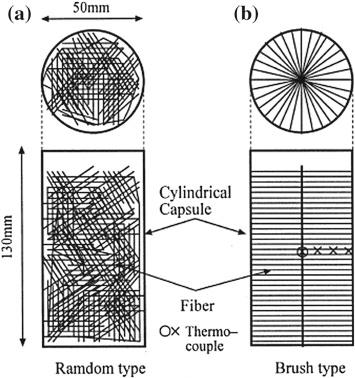
\includegraphics[scale=0.5]{images/configurationofthecarbonnanofibers.jpg}
\caption{Konfiguration von Carbon Nanofibers, In Abbildung a) ist es unstrukturiert und in b) ist es strukturiert eingebaut. \cite{WasteEnergyHarvesting}}
\label{fig:configurationofthecarbonnanofibers}
\end{center}
\end{figure}

Zusammengefasst die Zahl und Formen von PCM Speichern sollte optimiert werden
und es gibt noch keine klaren Ergebnisse und deshalb wird es weitere Studien
dazu geben.
Eine andere Möglichkeit wäre der Phasenübergang von gasförmig zu flüssig zu
verwenden, hier wäre das Fluid immer Flüssig und somit gut förderbar bzw. durch
die eigene Konvektion besser als das feste Material.


\subsection{Chemischer Speicher}
Gleich vorweg, im Gegensatz zu sensiblen oder latenten Wärmespeichern die
bereits kommerziell erhältlich sind, sind die Chemische Speicher bislang nur
Gegenstand der Forschung \cite{gegenstandderforschung}. So oder so soll in
diesem Kapitel näher darauf eingegangen werden. Die Wichtigsten Gründe weshalb
chemische Speicher sehr geeignet wären.
\begin{itemize}
\item Speicherung grosser Wärmemengen, da eine hohe Energiedichte 
\item Grosses Spektrum von verfügbaren Temperaturen
\item Specherung über lange Zeiträume ohne nennenswerte Verluste
\end{itemize}

\subsubsection{Arbeitsprinzip}
Bei der thermochemischen Speicherung werden chemische Reaktionen genutzt um
Wärme in einem Material zu speichern. Das Arbeitsprinzip dieser Speicher ist in
Abbildung \ref{fig:ladenspeichernentladens} ersichtlich. Wenn dem Material Wärme
zugeführt wird, wird es in zwei Komponenten zerlegt. Diese beiden Komponenten
können für lange Zeit ohne Energieverlust gespeichert werden. Werden diese
beiden wieder zusammengebracht, so findet die Umkehrreaktion statt und die Wärme
wird wieder frei.

\begin{figure}[h!]
\begin{center}
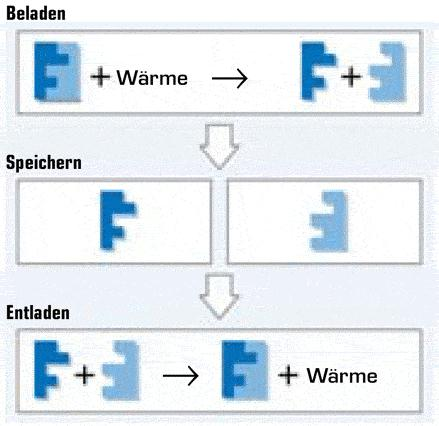
\includegraphics[scale=0.6]{images/ladenspeichernentladen.jpg}
\caption{Arbeitsprinzip \cite{ladenspeichernentladen}}
\label{fig:ladenspeichernentladens}
\end{center}
\end{figure}

Diese Prozesse werden mittels Sorption realisiert, wo sich unterteilen lässt in
Adsorbtion und Absorption. Diese können jeweils in einer offenes oder
geschlossenen Bauart umgesetzt werden.

\subsubsection{Stand der Technik der Adsorption}
Die Abbildung \ref{fig:adsorption} zeigt der Prozess einer geschlossenen
Adsorption. Technisch besteht so ein System hauptsächlich aus einem Porösen
Festkörper und einem gasförmigen Adsorptiv. Dabei gilt der Speicher als geladen,
wenn das Adsorptiv getrennt vom Adorbens ist. Durch das zusammenführen entsteht
Reaktionswärme welche genutzt werden kann. Ist das System entladen, muss
wiederum Wärme ins System gebracht werden, dass sich das gasförmige Adsorptiv
wieder löst und es getrennt gelagert werden kann.

\begin{figure}[h!]
\begin{center}
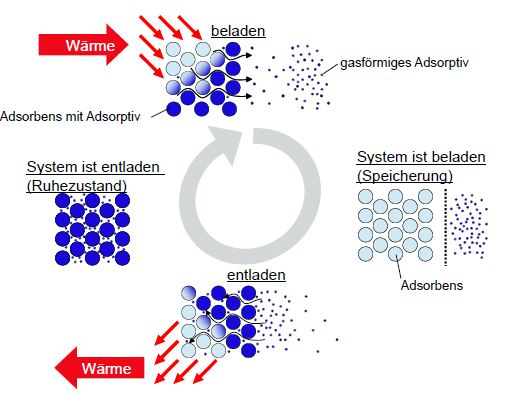
\includegraphics[scale=0.6]{images/prozess.jpg}
\caption{Prozess von Adsorption}
\label{fig:adsorption}
\end{center}
\end{figure}

Beim Laden des Speichers, siehe Abbildung \ref{fig:geschlossenerladen} wird
Wasser unter Wärmezufuhr aus Speichermaterial desorbiert. Die Kondensation des
Wasserdampf auf der passiert hier auf der linken Seite. Dabei muss gewährleistet
sein, dass $p_{v/k}$ < $p_R$ < 1bar ist.

\begin{figure}[h!]
\begin{center}
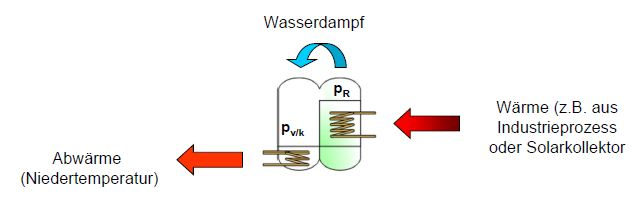
\includegraphics[scale=0.6]{images/geschlossenerladen.jpg}
\caption{Laden eines Geschlossenen Adsorptionssystem \cite{zeosys}}
\label{fig:geschlossenerladen}
\end{center}
\end{figure}

Bei der Entladung des Speichers wird das Wasser unter Vakuum verdampft. Es
passiert die Adsorption von Wasserdampfmolekülen am Speichermatierial und es
wird Wärme abgegeben. Dabei muss gewährleistet sein, dass 1bar > $p_{v/k}$ >
$p_R$ ist.


\begin{figure}[h!]
\begin{center}
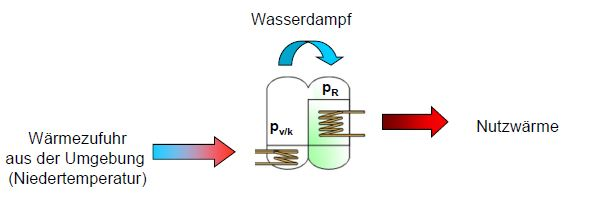
\includegraphics[scale=0.6]{images/geschlossenerentladen.jpg}
\caption{Entladen eines Geschlossenen Adsorptionssystem \cite{zeosys}}
\label{fig:geschlossenerentladen}
\end{center}
\end{figure}


Eine andere Möglichkeit ist die Adsorption mittels offenes System, welches in
der Abbildung \ref{fig:offenessystemadsorption} dargestellt ist. Diese
beinhaltet ein festen Adsorbentien (z.B. Zeolithen oder Silikagelen).  Bei der
offenen Adsorptionssystem transportiert der Luftstrom die Wärme und den
Wasserdampf in und aus einer Adsorbensschüttung. Somit werden die Lufttemperatur
und gleichzeitig der Wasserdampfpartialdruck des Luftstroms durch den
Sorptionsprozess beeinflusst. Die umgestzen Stoff- und Wärmemengen sind in der
\ref{fig:offenessystemadsorption} angedeutet.


\begin{figure}[h!]
\begin{center}
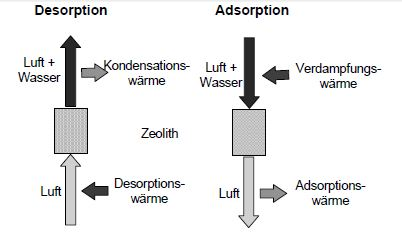
\includegraphics[scale=1]{images/offenessystemadsorption.jpg}
\caption{Offenes Absorptionssystem mit flüssigem Absorbens}
\label{fig:offenessystemadsorption}
\end{center}
\end{figure}




\subsubsection{Stand der Technik der Absorption}

Ähnlich lässt sich ein offenes Absorptionssystem beschreiben, siehe Abbildung \ref{fig:offenessystemabsorption}. Dabei wird jedoch mit flüssigen Absorbentien (wässerigen Salzlösungen, z.B. Lithiumchlorid oder Calciumchlorid) realisiert werden. Bei der Desorption wird verdünnte Salzlösung durch heisse Luft wieder konzentriert und der ausgetriebene Wasserdampf wird mit dem Luftstrom abtransportiert. Die konzentrierte Lösung kann bei der folgenden Absorption einen Luftstrom entfeuchten. Dabei wird sie wieder verdünnt. Die entfeuchtete Luft kann durch einen nachgeschalteten Befeuchter abgekühlt und zur Klimatierung eingesetzt werden. Die gespeicherte Energie lässt sich aus der Konzentrationsdifferenz der konzentrierten und verdünnten Lösung bestimmen. Da flüssige Absorbentien im Allgemeinen über deutlich geringere Bindungskräfte als feste Adsorbetien verfügen, wird bei der Absorption die entfeuchtete Luft vergleichsweise wenig erhitzt. Daher sind diese Speicher für den Einsatz in Heizanwendungen weniger oder nicht geeignet.

\begin{figure}[h!]
\begin{center}
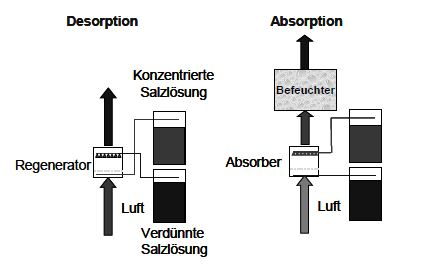
\includegraphics[scale=1]{images/offenessystemabsorption.jpg}
\caption{offenen Absorptionssystem}
\label{fig:offenessystemabsorption}
\end{center}
\end{figure}


Zum Bereich mit der Absorption des geschlossenen System konnten keine Informationen gefunden werden. Dies wird jedoch in einer Wärmepumpe eingesetzt, ist aber kein wirklicher Speicher.


\subsubsection{Entwicklung und Herausforderungen}
Unter den vielen Speicherformen hat die thermochemische Wärmespeicherung die theoretisch höchste Wärmespeicherdichte der unterschiedlichen Speicherform und weisst beinahe keine Verluste bei der Speicherung auf. Die Materialentwicklung und Systemintegration steckt derzeit jedoch noch in den Kinderschuhen. 
Die Forschung konzentriert sich derzeit auf die Entwicklung von leistungsfähigen, preiswerter und zyklenstabiler Materialen. Es müssen auch Konzepte gefunden werden für Speicher um die entstehenden Sorptionswärmen möglichst schnell abzuführen und wie dies im Gebäude integriert werden soll ist auch noch offen. Möglicherweise wäre es sogar denkbar solche Speicher zu transportieren um die Wärmeenergie Produktionsort und Verbraucherort sich nicht vereinbaren lassen.

\subsubsection{Perspektiven}
Das Spektrum möglicher Einsatzgebiete für Sorptionsspeicher ist breit, dies vor allem so, weil offene und geschlossene Speichersystemen zur Verfügung stehen in ganz verschiedenen Temperaturbereichen. 




\newpage
\section{Einsatzgebiete}
\subsection{Chemische Speicher im Gebäudeenergieeinsatz}
Da chemische Speicher die höchsten Energiedichten aller Speichertechnologien
aufweisen sind diese insbesondere stossen diese insbesondere auf Interesse in
der Gebäudetechnik. Die Speicher ermöglichen auch eine fast verlustfreie
Möglichkeit thermische Energie zu speichern. Diese beiden Eigenschaften machen
die Technologie für saisonale und kurzzeitige Anwendungen interessant.

\subsubsection{Kurzeitspeicher}

In einem Pilotprojekt hat das Bayrische Zentrum für angewandte Energieforschung
die technische Realisierung eines chemischen Speichers zum Lastenausgleich in
einem Fernwärmenetz beweisen können. Der thermochemische Zeolithspeicher wurde
erfolgreich im Heizsystem einer Münchner Schule integriert. In der Nacht bei
geringer Last wird der Speicher aufgeladen und bei normaler Tageslast entladen.
Untertags ist es mit diesem System möglich, eine komplette Abkopplung vom
Fernwärmenetz vorzunehmen und nur über den chemischen Speicher zu heizen. Der
Speicher ist so ausgelegt, dass er die Heizlast von 95kW über 14 Stunden liefern
kann. Technisch gesehen besteht der Speicher aus drei Kammern die total 1700kg
Zeolith 13X entahlten. Der Arbeitsbereich von Zeolith 13X ermöglicht ein Laden
bei 130\textdegree C und ein Entladen bei ca. 110\textdegree C. Technisch
gesehen kommt ein Adsorptionsspeicher mit kombinierter Wärmepumpe zum Einsatz:

In der Nacht wird durch Fernwärme auf 130\textdegree C erwärmte Luft durch den
Zeolithspeicher geleitet. Die trockene Luft nimmt das an den Zeolith gebundene
Wasser auf und wird auf einem tieferen Temperaturniveau durch einen Kondensator
geleitet. Dabei entsteht Kondensationswärme auf einem Niveau von 40\textdegree C
welche für einen Nachtbetrieb der Heizung geeignet ist. 

Untertags entladen wird der Speicher indem das Kondensat auf niedrigem
Temperaturniveau wieder verdampft und diese Luft dann durch den Speicher
geleitet wird. Der dabei ablaufende Adsorptionsprozess setzt Hochtemperaturwärme
frei.In Abbildung \ref{fig:Laden} und \ref{fig:Entladen} ist das Prinzipschema
der Anlage abgebildet.

\begin{figure}[h!]
\begin{center}
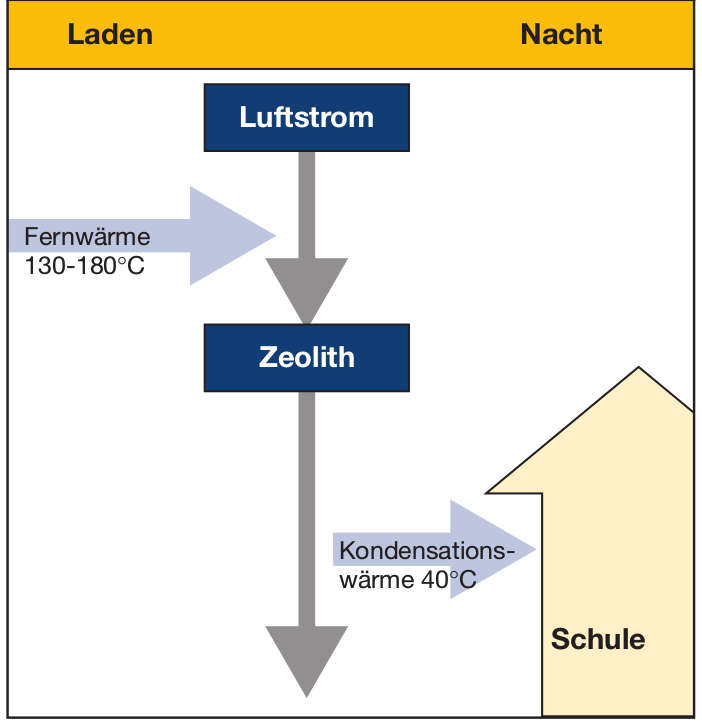
\includegraphics[scale=1]{images/Laden.jpg}
\caption{Laden des Zeolithspeichers \cite{BINE2}}
\label{fig:Laden}
\end{center}
\end{figure}

\begin{figure}[h!]
\begin{center}
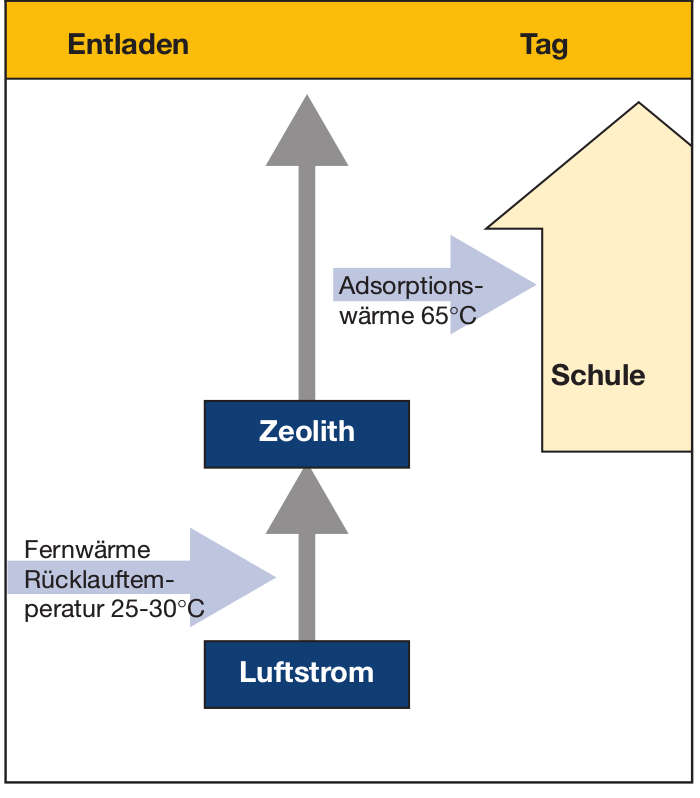
\includegraphics[scale=1]{images/Entladen.jpg}
\caption{Entladen des Zeolithspeichers \cite{BINE2}}
\label{fig:Entladen}
\end{center}
\end{figure}
Experimentell konnte ein Speicherwirkungsgrad von 86\% nachgewiesen werden.
Nachteilig erwiesen sich der hohe Preis von Zeolith der verhältnismässig hohe
Inverstitionskosten verursachte. Eine Ammortisation bei einem Betrieb mit 100
Zyklen pro Jahr scheint innert 10-15 Jahren möglich. Unter Laborbedingungen
verliert das Zeolith nach 100 Ladezyklen 15\% der Adsoprtionsenthalpie.
Anschliessend scheint die Adsorptionsfähigkeit des Stoffs stabil zu bleiben.
Dies ist ebenfalls in der Wirtschaftlichkeitsberechnung zu berücksichtigen.
\cite{BINE2}

\subsubsection{Saisonaler Speicher}
Saisonale thermochemische Speicher sind ebenfalls möglich. Das Fraunhofer-
Institut für solare Energiesysteme zusammen mit UFE Solar GmbH eine
Sorptionsspeicher für Niedrigenergiehäuser. Im Sommer word der Sorptionsspeicher
mittels thermischer Solarkollektoren aufgeladen und im Winter das Haus über den
Sorptionsspeicher mit thermischer Energie versorgt. Für Spitzenlastzeiten wurde
eine Zusatzheizung eingebaut. Als Speichermaterial wird handelsübliches
Silicagel verwendet. Technisch gesehen kommt auch hier ein Adsorptionsspeicher
mit kombinierter Wärmepumpe zum Einsatz. Das Prinzipschema ist in Abbildung \ref{fig:Saisonaler Speicher}
abgebildet.

\begin{figure}[h!]
\begin{center}
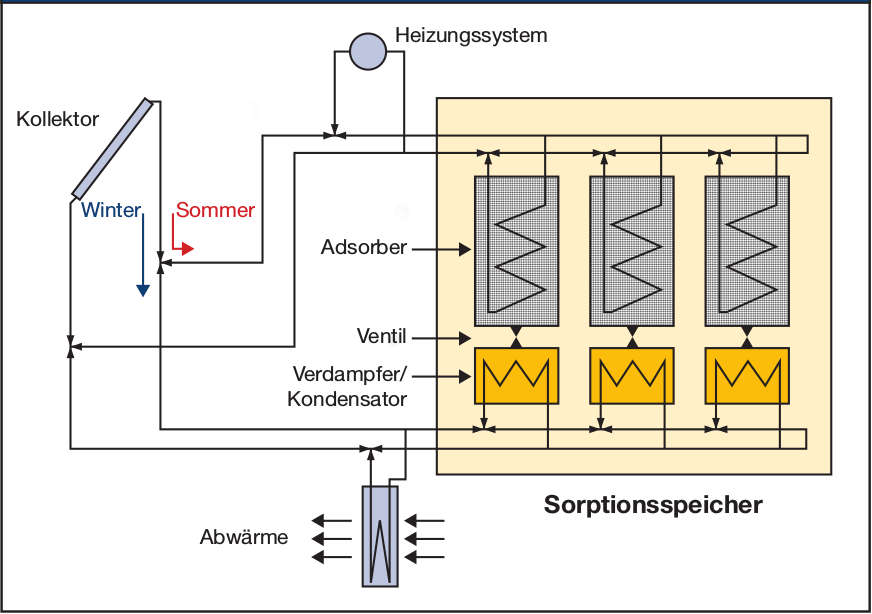
\includegraphics[scale=1]{images/energiehaus.jpg}
\caption{Schema des saisonalen chemischen Speichers \cite{BINE2}}
\label{fig:Saisonaler Speicher}
\end{center}
\end{figure}

Um einen möglichst flexiblen Einsatz mit gleichzeitiger Be- und Entladung zu
ermöglichen ist die geschlossen funktionierende Anlage drei Mal mit allen
Komponenten ausgestattet. Das Kondensat wird in dafür geeigneten Behältern
aufbewahrt. 

Anhand einer Simulation wurde die geschätzte Heizleistung von 4000kWh\/a mit
32m$^2$ thermischen Solarkollektoren und einem Sorptionsspeicher von 11m$^3$
Volumen veranschlagt bei 100\% Deckungsgrad. Ein Kostenoptimum für den solaren
Deckungsgrad mit Zusatzheizung wurde für eine Auslegung 80-90\% prognostiziert.

Zum Zeitpunkt der Publikation von \cite{BINE2} befindet sich der Speicher noch
in Evaluation. Insbesondere der tatsächlich erreichbare solare Deckungsgrad wäre
dabei von Interesse. Leider liessen sich im Internet keine aktualiserten
Resultate zu diesem Projekt finden.
\subsection{Latentspeicher}
Die Zürcher Firma GLASSX stellt PCM Fassadenelemente her. 

Kernprodukte sind
GLASSX\circledR store, ein kombinierbares Innenelement für Gebäude mit
Glassfassade und GLASSX\circledR crystal, ein Komplettfasadenelement mit
Verschattung und Dämmung für Leichtbaugebäude. Die beiden Produkte besitzen eine
ähnlichen Aufbau. Das PCM, Kalziumchloridhexahydrat (\ce{CaCl_2\cdot 6H_2O}),
liegt zwischen zwei Gläsern in der Mitte des Elements. Der Schmelzpunkt von
\ce{CaCl_2\cdot 6H_2O} liegt genau bei Raumtemperatur (Salzhydrat). Bei
Erwärmung durch Sonneneinstrahlung schmilzt das \ce{CaCl_2\cdot 6H_2O} und
entzieht so der Umgebung Wärme. Bei Abkühlung in der Nacht gestaltet sich der
Prozess genau umgekehrt. \ce{CaCl_2\cdot 6H_2O} erstarrt und gibt Wärme an die
Umgebung ab. Da diese Elemente als Fassade bzw. direkt hinter der GLasfassade
eingesetzt werden, wird bicht nur Raumwärme sondern auch die Einstrahlungswärme
der Sonne genutzt. Infrarotstrahlung wird durch das PCM fast komplett
absorbiert, für sichtbares Licht ist das Material zum grössten Teil durchlässig.
Als weitere Innovation hat das Unternehmen ein Prismenglas entwickelt, dass die
unterschiedlichen Einstrahlungswinkel während der Jahreszeiten als Selektion
nutzt. Bei hohen Einstrahlungswinkeln wie sie im Sommer vorkommen wird über
Totalreflexion der grösste Teil der Strahlung bereits im Prismenglas absorbiert.
Im Winter bei niedrigeren Einstrahlungswinkeln lässt das Glas die Strahlung
annähernd verlustfrei durch. Somit sind im Winter solare Gewinne möglich. In
Abbildung \ref{fig:glassx schema} ist das Schema einer GLASSX\circledR crystal
Fassade mit Prismenglas abgebildet. 

\begin{figure}[h!]
\begin{center}
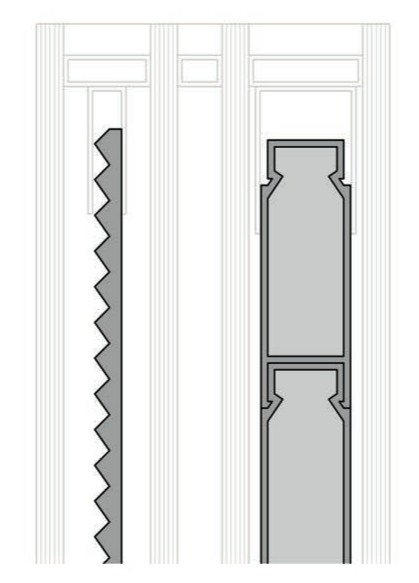
\includegraphics[scale=0.7]{images/glassxcrystal.jpg}
\caption{Schema einer GLASSX\circledR crystal Fassade \cite{glassxbr}}
\label{fig:glassx schema}
\end{center}
\end{figure}

Der Autor konnte sich im Referenzgebäude von Marché Schweiz selber auf einer
Exkursion von der Funktionalität der Elemente überzeugen. Die Wirkung dieser
Bauteile ist bestechend. Das Raumklima blieb ohne zusätzliche Verschattung
selbst im Hochsommer angenehm. Als Ergänzung zu den baulichen Massnahmen wurde
die Luftbefeuchtung mit speziellen Wasserpflanzen gewährleistet. 
\newpage
\section{Ausblick}
\newpage
\listoftables
\newpage
\listoffigures
\newpage
\begin{thebibliography}{99}
	\bibitem{BINE1}BINE Energieforschung für die Praxis. Abgerufen am 11.04.2014
	
	von http://www.bine.info/typo3temp/pics/b193b0972c.gif verändert durch D. Strebel
	\bibitem{Wesselak}Wesselak et. al. Regenerative Energiesysteme. 2. Auflage.
	Springer Vieweg Verlag Berlin. 2013
	
	\bibitem{Hiebler} Hiebler S. Kalorimetrische Methoden zur Bestimmung der
	Enthalpie von Latentwärmespeichermaterialien während des Phasenübergangs. Dissertation.
	München. 2007
	
	\bibitem{BINE2} BINE Energieforschung für die Praxis. projektinfo 2\/01
	Thermochemische Speicher. 2001
	
	\bibitem{glassxbr} GLASSX\circledR crystal. Das Glas, das speichert, wärmt und
	kühlt. Produktbroschüre. Zürich. 2005.
	 
	\bibitem{Phasendiagramm} Wikipedia Phasendiagramm. 
	Abgerufen von
	
	http//commons.wikimedia.org/wiki/File:Phasendiagramme.svg am 28.04.2014.
	Verändert von D.Strebel
	
	\bibitem{Henning} Henning H.M. Phasenwechselmaterialien in Baumaterialien und
	Leitungssystemen. Präsentation. Fraunhofer Institut für solare Energiesysteme,
	Freiburg. 2007
	
	\bibitem{Gschwander} Gschwander S. et al. Micro-encapsulated paraffinin
	phase-change slurries. Fraunhofer Institut für solare Energiesysteme,
	Freiburg. Elsevier Verlag. 2005

	\bibitem{BINE3} BINE Energieforschung für die Praxis. Projektinfo 16/2012.
	Pahsenübergang speichert Wärme. 2012
		
	\bibitem{meltingpaper} Constrained and unconstrained melting inside a sphere. Available online at www.sciencedirect.com. 2007
	
	\bibitem{WasteEnergyHarvesting} Waste Energy Harvesting, Mechanical and Thermal Energies, Volume 24.
		Springer Vieweg Verlag Berlin. 2014
		
	\bibitem{gegenstandderforschung} Technische Universität München. TcET – Thermochemischer Energiespeicher für thermische Kraftwerke und industrielle Wärme.
	Abgerufen von http://www.es.mw.tum.de/index.php?id=322 am 03.05.2014		
		
	
	\bibitem{ladenspeichernentladen} Erneuerbare Energie. 
	Abgerufen von http://www.aee.at am 03.05.2014
	
	
    \bibitem{zaebayern} ZAE BAYERN. Abgerufen von http://www.wuerzburg.ihk.de am 03.05.2014	% http://www.wuerzburg.ihk.de/fileadmin/user_upload/pdf/Innovation_Umwelt/Vortraege/Dr._Hauer-Thermische_Energiespeicher.pdf
    
    \bibitem{zeosys} ZeoSys Gmbh. Dr.Asnakech Lass-Seyoum. Kolloquium Effiziente Energienutzung. Stuttgard, 03. Juli 2013
	
\end{thebibliography}
\end{document}
